\documentclass[a4paper,twoside,12pt,chapterprefix=false]{scrbook}

\usepackage{amsmath,amssymb,amsthm}
%\usepackage[footnotesize,sl,SL,hang,tight]{subfigure}  % helpful package for aligning figures next to each other
\usepackage{longtable} % tables over several pages
\usepackage[font={small,sl},hang,labelfont=bf]{caption} % configure captions
%\usepackage{captcont} % continue sufigures over several pages
\usepackage{booktabs} % publication quality tables for LaTeX
%\usepackage{showkeys} % shows the labels above the references for easier development

\ifpdfoutput{%
	\usepackage[pdftex]{graphicx}
	\usepackage[]{pdfpages} %for including full pdf pages
}{%
	\usepackage{graphicx}
}
\usepackage{rotating} % rotate figures

\usepackage{scrpage2}
\KOMAoptions{headinclude}

\usepackage{caption}
\usepackage{subcaption}

% Font packages:
\usepackage{times}
\usepackage{helvet}   % sets sans serif font
\usepackage[T1]{fontenc}

%PDF hyperref config
\ifpdfoutput{%
	\usepackage[pdftex,
		bookmarks,
		bookmarksopen=true,
		bookmarksnumbered=true,
		pdfauthor={My Name},
		pdftitle={Thesis Title},
		colorlinks,
		linkcolor=black,
		citecolor=black,
		filecolor=black,
		urlcolor=black,
		anchorcolor=black,
		menucolor=black,
		breaklinks=true,
		pageanchor=true,
		plainpages=false,
		pdfpagelabels=true]{hyperref}
}{}

\ifpdfoutput{%
	\pdfcompresslevel=9
	\pdfoutput=1
	\DeclareGraphicsExtensions{.pdf,.png}
}{}

\bibliographystyle{alpha}

% Uncomment the chapter / section you are working on.
%
%\includeonly{figures}
%\includeonly{tables}
%\includeonly{data-analysis}
%\includeonly{conclusion}
%\includeonly{apx-sample-appendix}

%\pagestyle{useheadings}

% A4
%
\topmargin -0.5in
\textheight 9.3in
\textwidth 6.3in
\oddsidemargin 0.18in
\evensidemargin -0.22in
\parskip 0.1in
\parindent 0in

\renewcommand{\arraystretch}{1.5}
\renewcommand{\baselinestretch}{1}

% commands
\newcommand{\Adjoint}{\mbox{\rm Adj}}
\newcommand{\Area}{\mbox{\rm Area}}
\newcommand{\ACos}{{\mbox{\rm Cos}^{-1}}}
\newcommand{\ASin}{{\mbox{\rm Sin}^{-1}}}
\newcommand{\ATan}{{\mbox{\rm atan2}}}
\newcommand{\Code}[1]{{\tt #1}}
\newcommand{\Complex}{\mbox{\bf C}}
\newcommand{\Cross}{{\mbox{\rm Cross}}}
\newcommand{\Mydddot}[1]{\mbox{\shortstack{$.$\hspace*{-1pt}$.$\hspace*{-1pt}$.$\\$#1$}}}
\newcommand{\Degree}{\mbox{\rm degree}}
\newcommand{\Diag}{\mbox{\rm Diag}}
\newcommand{\Dim}{\mbox{\rm dim}}
\newcommand{\Dist}{\mbox{\rm Distance}}
\newcommand{\IntTwo}{\int\!\!\int}
\newcommand{\IntThree}{\int\!\!\int\! \!\int}
\newcommand{\Kernel}{\mbox{\rm kernel}}
\newcommand{\Kross}{\mbox{\rm Kross}}
\newcommand{\Grad}{\nabla}
\newcommand{\Perp}{\mbox{\rm Perp}}
\newcommand{\Point}[1]{{\cal #1}}
\newcommand{\Rank}{\mbox{\rm rank}}
\newcommand{\Range}{\mbox{\rm range}}
\newcommand{\Real}{{\mbox{\rm I}\hspace*{-2pt}\mbox{\rm R}}}
\newcommand{\RealSbt}{{\mbox{\rm\scriptsize I}\hspace*{-2pt}\mbox{\rm\scriptsize R}}}
\newcommand{\Res}{\mbox{\rm resultant}}
\newcommand{\Sbt}[1]{{\mbox{\rm\scriptsize #1}}}
\newcommand{\MySign}{\mbox{\rm Sign}}
\newcommand{\SignSBT}{\mbox{\rm\scriptsize Sign}}
\newcommand{\Skew}{\mbox{\rm Skew}}
\newcommand{\Span}{\mbox{\rm Span}}
\newcommand{\SqrDist}{\mbox{\rm Distance$^2$}}
\newcommand{\Trace}{\mbox{\rm Trace}}
\newcommand{\TRN}{{\mbox{\rm\scriptsize T}}}
\newcommand{\Vector}[1]{\mbox{\bf #1}}
\newcommand{\VectorM}[1]{\mbox{\boldmath $#1$}}
\newcommand{\Volume}{\mbox{\rm Volume}}

\newcommand{\IVec}{\mbox{\boldmath $\imath$}}
\newcommand{\JVec}{\mbox{\boldmath $\jmath$}}
\newcommand{\KVec}{\mbox{\boldmath $k$}}
\newcommand{\LVec}{\mbox{\boldmath $\ell$}}
\newcommand{\RMat}{{\cal R}}
\newcommand{\QMat}{{\cal Q}}
\newcommand{\QCMat}{\overline{\cal Q}}

\newcommand{\Lerp}{\mbox{\rm lerp}}
\newcommand{\Slerp}{\mbox{\rm slerp}}
\newcommand{\Quad}{\mbox{\rm quad}}
\newcommand{\Squad}{\mbox{\rm squad}}

\newcommand{\subsubsubsection}[1]{{\sc #1}}

\newcommand{\ODer}[2]{\frac{d #1}{d #2}}
\newcommand{\ODerT}[2]{\frac{d^2 #1}{d {#2}^2}}
\newcommand{\ODerM}[3]{\frac{d #1}{d #2 \, d #3}}
\newcommand{\PDer}[2]{\frac{\partial #1}{\partial #2}}
\newcommand{\PDerT}[2]{\frac{\partial^2 #1}{\partial {#2}^2}}
\newcommand{\PDerM}[3]{\frac{\partial^2 #1}{\partial #2 \, \partial #3}}

% mass density symbol
\newcommand{\Den}{\delta}

% environments
\newenvironment{BArray}[1]{\left\{ \begin{array}{#1}}{\end{array} \right\}}
\newenvironment{Combin}{\left( \begin{array}{c}}{\end{array} \right)}
\newenvironment{Matrix}[1]{\left[ \begin{array}{#1}}{\end{array} \right]}

% "Figure" environment
\newtheorem{localFigure}{Figure}[chapter]
\newenvironment{Figure}[1]{
  \begin{center}
  \begin{minipage}{6in}
  \par\noindent\hspace*{0pt}\hrulefill
  
  \begin{localFigure} \label{#1}
}{
  \end{localFigure}
  \par\noindent\hspace*{0pt}\hrulefill
  \end{minipage}
  \end{center}
}

% "Table" environment
\newtheorem{localTable}{Table}[chapter]
\newenvironment{Table}[1]{
  \begin{center}
  \begin{minipage}{6in}
  
  \begin{localTable} \label{#1}
}{
  \end{localTable}
  \end{minipage}
  \end{center}
}

% "CDROM" environment for source code on disk
%\newenvironment{CDROM}[1]{
%  \label{#1} 
%    \includegraphics{cdrom.png} \hspace*{0.1in}{\tt PointShop3D}. \rm
%}{
%  $\bowtie$
%}

% TO DO search symbol
\newcommand{\TODO}{\mbox{\large\bf TO DO}}
\newcommand{\REFR}{\mbox{\large\bf REFR}}

%  Terminates current page and paragraph, makes sure next page starts on
%  an odd-number, and generates a completely blank page, without page markers,
%  if necessary.
\newcommand{\clearemptydoublepage}{\newpage{\pagestyle{empty}\cleardoublepage}}

%%% Shoemake's commands
\DeclareMathOperator{\prp}{\text{\scshape perp}}
\DeclareMathOperator{\rot}{rot}
\DeclareMathOperator{\N}{N}
\providecommand{\vmag}[1]{\lVert#1\rVert}
\providecommand{\mutate}[1]{\overleftarrow{#1}}
\providecommand{\T}[1]{{#1}^{\mathrm T}}
\newcommand{\cross}{\times}
\newcommand{\by}{\times}
\newcommand{\vect}[1]{\mathbf{#1}}
\newcommand{\mat}[1]{\mathbf{#1}} % or not
%\newcommand{\quat}[1]{\mathbf{#1}}
\newcommand{\quat}[1]{\ensuremath{\mathbf{\dot{#1}}}}
\newcommand{\vV}{\vect{v}}
\newcommand{\vU}{\vect{u}}
\newcommand{\vE}{\vect{e}}
\newcommand{\vUh}{\hat{\vect{u}}}
\newcommand{\mQ}{\mat{Q}}
\newcommand{\mR}{\mat{R}}
\newcommand{\mM}{\mat{M}}
\newcommand{\mA}{\mat{A}}
\newcommand{\mB}{\mat{B}}
\newcommand{\mI}{\mat{I}}
\newcommand{\mJ}{\mat{J}}
\newcommand{\mX}{\mat{X}}
\newcommand{\mY}{\mat{Y}}
\newcommand{\mZ}{\mat{Z}}
\newcommand{\qo}{\quat{1}}
\newcommand{\qi}{\quat{i}}
\newcommand{\qj}{\quat{j}}
\newcommand{\qk}{\quat{k}}
\newcommand{\xh}{{x}}
\newcommand{\yh}{{y}}
\newcommand{\zh}{{z}}
\newcommand{\ch}{c}
\newcommand{\sh}{s}
\newcommand{\gt}{\theta}


%%
%%
%%


\begin{document}

%% Define leading chapter pages
%
%\addtokomafont{chapter}{\setlength{\parskip}{190pt}}   % SEVERE HACK to keep spacing to chapter art work
\renewcommand*{\chapterheadstartvskip}{\vspace*{215pt}}  % different hack to keep spacing to chapter artwork
%\addtokomafont{chapter}{\rmfamily}        % remove this if you prefer sans-serif section titles
%\addtokomafont{section}{\rmfamily}        % remove this if you prefer sans-serif section titles
%\addtokomafont{subsection}{\rmfamily}     % remove this if you prefer sans-serif section titles
%\addtokomafont{subsubsection}{\rmfamily}  % remove this if you prefer sans-serif section titles
%\addtokomafont{paragraph}{\rmfamily}      % replace by \sffamily if you prefer sans-serif para titles
\addtokomafont{paragraph}{\sffamily}

\def\mychpstyleintl{%
{\noindent\setlength{\tabcolsep}{0pt}\setlength{\arrayrulewidth}{2pt}%
\begin{tabular}{c}
\\[100pt]
\begin{tabular}{lr}
\begin{tabular}{p{0.6\linewidth}}
\\
\end{tabular}
&
\begin{tabular}{p{0.4\linewidth}}
\rightline{{%
\sffamily%
\fontseries{bx}%
\fontshape{n}%
\fontsize{100}{120}%choose baselineskip to be 1.2 times font size
\selectfont
\thechapter}}
\end{tabular}
\end{tabular}\\[300pt]
\end{tabular}
}}

\newpagestyle{mychapterpagestyle}{{\protect\mychpstyleintl}{\protect\mychpstyleintl}}{}
\newpagestyle{myappendixpagestyle}{{\protect\mychpstyleintl}{\protect\mychpstyleintl}}{}
%%

%% macros e.g.
\newcommand{\mfytext}[0]{my fancy text}

%refs
\newcommand{\chpref}[1]{Chapter \ref{#1}}
\newcommand{\secref}[1]{Section \ref{#1}}
%\newcommand{\equref}[1]{Equation \ref{#1}} %better use builtin \eqref{}
\newcommand{\figref}[1]{Figure \ref{#1}}
\newcommand{\tabref}[1]{Table \ref{#1}}
\newcommand{\apxref}[1]{Appendix \ref{#1}}
%%

\hypersetup{pageanchor=false} % disabling anchors for title page to avoid warning

%% Replace this by your own design of a title page
%
%\title{Thesis Title}
%\author{My Name}
%\date{September 2042}
%\maketitle
%\clearemptydoublepage
% --- selfmade version ----
\begin{titlepage}
	\topmargin 1.0cm
	\oddsidemargin 0.0cm
	\evensidemargin 0.0cm
	%\textwidth 6.5in
	\centering
	\Huge
	\vspace{3.0cm}
	\textbf{\textsf{Inferring Human Body Parts and Correlations from Images, Pointclouds and Meshes}} \\[2.0cm]
	%\includegraphics*[width=0.4\textwidth]{figures/titlefigure} \\[4.0cm]
	\vspace{5.0cm}
	\sffamily
	\Large
	David Haldimann
	\\[0.8cm]
	\large
	Semester Thesis
	\\
	June 2018
	\\[1.3cm]
	Prof. Dr. Markus Gross
	\vfill
	\includegraphics*[width=0.3\textwidth]{figures/ETH_logo} \hfill
	\includegraphics*[width=0.3\textwidth]{figures/CGL_logo}
	\vspace{3.4cm}
\end{titlepage}
\clearemptydoublepage
%%

\hypersetup{pageanchor=true}
\pagenumbering{roman}
\setcounter{page}{1}

\chapter*{Abstract}

This thesis addresses the development of a novel sample thesis. We analyze the requirements of a general template, as it can be used with the \LaTeX\ text processing system. (And so on\dots) The abstract should not exceed half a page in size!

\cleardoublepage
\chapter*{Zusammenfassung}

Diese Arbeit besch�ftigt sich mit der Entwicklung einer neuartigen Beispielausarbeitung. Wir untersuchen die Anforderungen, die sich f�r eine allgemeine Vorlage ergeben, die innerhalb der \LaTeX-Textverarbeitungsumgebung verwendet werden kann. (Und so weiter und so fort\dots) Die Zusammenfassung sollte nicht l�nger als eine halbe Textseite sein!


%include task description here:
\cleardoublepage
%\includegraphics[viewport=3cm 0cm 20cm 27.5cm]{task_description} %better use includepdf below!
%\includepdf{task_description}
\cleardoublepage

%include acknowledgment here:
%\include{acknowledgment}

\tableofcontents
\cleardoublepage

\addcontentsline{toc}{chapter}{List of Figures}
\listoffigures
\cleardoublepage

\addcontentsline{toc}{chapter}{List of Tables}
\listoftables
\cleardoublepage

\pagenumbering{arabic}
\renewcommand*{\chapterpagestyle}{mychapterpagestyle}
\renewcommand*{\chapterformat}{} % show chapter titles only (no numbers)
% \setchapterpreamble[o]{...}  unfortunately does not move the \chapter output downwards

% ---- MAIN PART ----

% set counter to n-1:
\setcounter{chapter}{0}

\chapter{Introduction}

The price for breast enhancement surgery was estimated to be \$3718 in 2017 according to the American Society of Plastic Surgery\footnote{https://www.plasticsurgery.org/cosmetic-procedures/breast-augmentation/cost}. Next to the financial aspects, there are also risks connected to undergoing surgery as well as not knowing exactly what the result will look like. Before commiting to this kind of operation, it should be possible to generate a preview of the outcome from a few images. This thesis aims to design a method that is able to predict a 3D model of the outcome by learning a mapping between parametric models. Additionally, the idea is explored, if it is possible to generate a parametric model from a character modelling software.

%https://www.plasticsurgery.org/cosmetic-procedures/breast-augmentation/cost



\section{Parametric Model}
A previous implementation by Biland \cite{Biland17} was used to create parametric models. A parametric model can describe all data that went into the model with its parameters. For example, the physical appearance of a person can be roughly described by their height, skin tone and hair color, where these three are the parameters of this parametric model. This is, of course, only an approximation as the accuracy of the description of the person would increase with more parameters. It is also possible, that one parameter influences multiple features. In the previous example, when the height of a person is raised, the length of the arms are also proportionally increased.

\section{Mapping}
A mapping between sets associates each element in the first set with one or more elements of the second set. An example for a simple mapping could be the numbers one to twenty-six as the first set and the letters of the alphabet as the second. In the case of two parametric models, the goal is to find a mapping that describes the relationship between the parameters of the first and second model. \\
This mapping can either be linear or non-linear. The difference between a linearity and a non-linearity can be described with a simple example. The time it takes to drive $10km$ in a car at $10\frac{km}{h}$ is $1h$. If the distance to drive is doubled to $20km$, so will the time it takes. That is, because distance to drive and time it requires are in a linear relationship. On the other hand, given that the braking distance while travelling with $10\frac{km}{h}$ is $1m$, the braking distance while travelling with $20\frac{km}{h}$ is $4m$. This is due to the fact, that speed and braking distance are related in a quadratic, non-linear, manner.

\section{Applications}
The applications for this method could be plenty. While the most obvious use for this implementation would be plastic surgery - creating 3D models from images of possible breast enhancements, it could also be used in oncology, to show affected patients what their body might look like after a mastectomy and even further, after a possible reconstruction. This approach could also be used in an adapted version for commercial use, such as tailor fitting clothes by using an image of the customer.

% set counter to n-1:
\setcounter{chapter}{1}

\chapter{Related Work}
In the field of modelling the human body, early on, a lot of work was done concerning the face. Jeng et al. \cite{jeng1998facial} proposed a geometric face model to localize the face in an image and detect facial features efficiently. The reason for the need of a functioning model for faces may have been the upcoming importance of faciel recognition.\\
Parametric models have also been applied to reshaping the human body in images using semantic parameters. \cite{zhou2010parametric} Their approach included reshaping a morphable 3D model and applying the reshaping effects using an image warping approach. Other work was done by Allen et al. \cite{allen2003space} on parametrizing full body scans and using the parameters in a variety of applications. One application was to find features connected to certain parameters, such that for example the weight could be increased and the resulting mesh would increase in size in a meaningful way.\\
Work about specifically modelling the breast has been done by Galle et al. \cite{gallo2010human}. They proposed a parameter space based on MRI scans to describe the shape of a human breast using PCA. Ciechomski et al. \cite{de2012development} proposed a web approach to create 3D models from images where participants uploaded images and selected keypoints. These 3D models can later be accessed by surgeons to visualize different types and sizes of implants applied.

\chapter{Methods}
In this chapter, the methods needed to create a parametric model and a mapping between parametric models are introduced and explained. Firstly, the data gathering and preprocessing are outlined. Multiple variants of the parametric model are discussed. Different learning approaches for the mapping are reviewed. Lastly, a character editor is presented that is used to generate data for a parametric model.

\section{Data Acquisition and Preprocessing}
It would be necessary to have a large data set of images of women before and after breast enhancement surgery, where the patients pose topless. It is very unlikely though, that such a database exists, due to the fact that having breast surgery is a very personal topic and people generally don't enjoy posing naked. Therefore, the images used were downloaded from a website\footnote{https://my.crisalix.com/} that offered to simulate various plastic surgical procedures including breast enhancement. For each user, a 3D model of their torso was displayed side by side with different enhancements varying in size. An screenshot of the interface can be seen in figure \ref{fig:websiteExample}.\\

\begin{figure}[h]
\centering
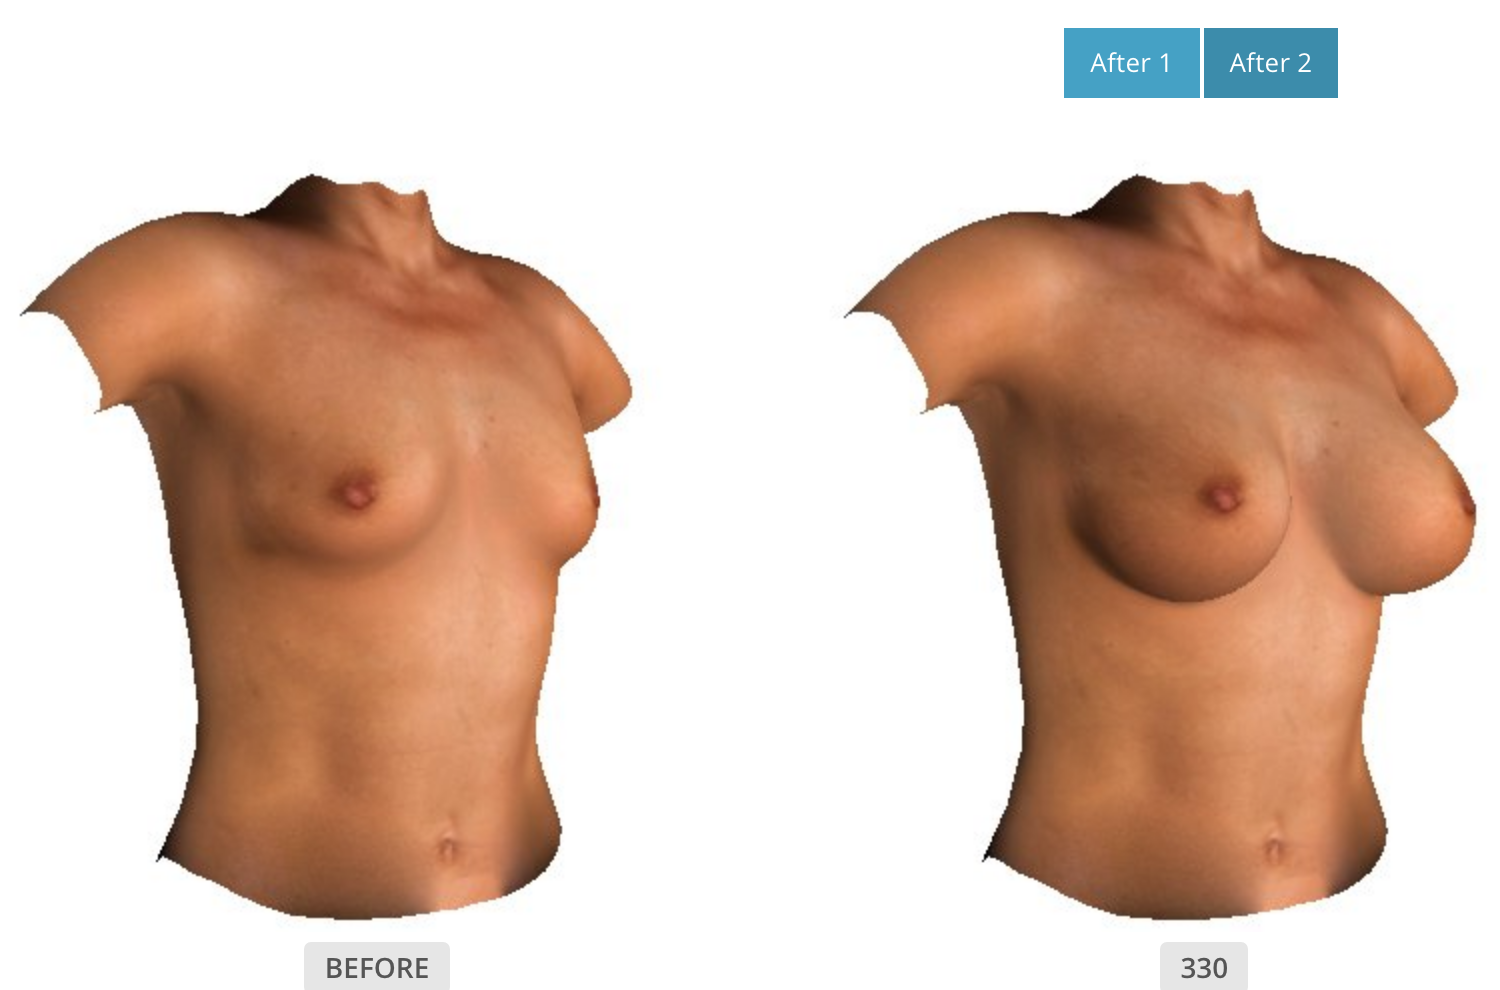
\includegraphics[width=0.75\textwidth]{figures/websiteExample}
\caption[Website UI example]{Example screenshot of the visualization on the website of Crisalix.}
\label{fig:websiteExample}
\end{figure}

Each model was made up of a sequence of 24 images displaying the torso from different angles. This dataset fit the requirements nicely, as images are available for \textit{before} and \textit{after}, except the \textit{after} is generated and based on their model. Additionally, each after image sequence had a short label, usually describing how much silicone was added, that was also saved for further evaluation. In total 2'937 examples were retrieved and preprocessed. This dataset included images from 748 subjects of which each one was comprised of one \textit{before} and at least one \textit{after} image sequence.\\

In a next step, these image sequences needed to be transformed into point clouds. This was done, using a general-purpose Structure-from-Motion (SfM) \cite{schoenberger2016sfm} and Multi-View Stereo (MVS) \cite{schoenberger2016mvs} pipeline called COLMAP. This generated point clouds, spanning from 5'000 to 15'000 points. Some of the images needed to be discarded, due to the fact that SfM created a point cloud with less than 1'000 points or the point clouds had holes, such that certain areas had no points and were not defined at all. The remaining point clouds were cleaned using a C++ implementation by Biland \cite{Biland17} that removed white points around the borders.

The mapping required to have one set of point clouds of \textit{before} examples and the corresponding\footnote{Corresponding meaning, based on the same subject.} \textit{after} examples. Therefore, the data was split into sets of \textit{before} and \textit{after} point clouds. As all of the \textit{after} point clouds were based on various breast enhancements, all the corresponding labels were processed and analyzed. This resulted in a table of terms sorted by the frequency of the term. The 9 most frequent terms can be found in table \ref{tableTerms}.

\begin{table}[h]
\centering
\begin{tabular}{|l|l|l|l|l|l|l|l|l|l|}
\hline
\textbf{Term}      & \textbf{R:} & \textbf{L:} & \textbf{LSC} & \textbf{73} & \textbf{cc} & \textbf{LSA} & \textbf{350} & \textbf{Custom} & \textbf{300} \\ \hline
\textbf{Frequency} & 205         & 205         & 100          & 85          & 54          & 73           & 73           & 70              & 60           \\ \hline
\end{tabular}
\caption[Table of most frequent terms]{The 9 most frequent terms can be seen in the upper row. The corresponding frequency is stated below.}
\label{tableTerms}
\end{table}

The first few terms are not informative, as they don't describe the breast themselves. The terms "LSC" and "73" are descriptions of a certain implant \footnote{http://www.simplybreastimplants.com/breast\_implant\_sizes/sebbin\_firm\_high\_profile.html} and "cc" is a measure of volume. The first meaningful term is "350", which means that an implant with a volume of 350ml was inserted. Therefore, only the \textit{after} examples that were labelled "350" were included, to create a better mapping. After removing some of the point clouds that were not reconstructed well enough, this resulted in 57 examples in the \textit{before} and 57 in the \textit{after} set. All of these point clouds were further processed in a MATLAB implementation by Biland \cite{Biland17} to generate mesh files using a method called nonrigid iterative closest point (NRICP) algorithm. Given a point cloud and a base mesh, NRICP iteratively deforms the base mesh to match the points in the point cloud. The parameters used in this thesis can be found in the appendix in table \ref{nricpParams} and the template mesh used was the Audrey mesh. This is one of the meshes that was also used by Biland.

\subsection{Alignment}
\label{align}
The meshes are aligned in the procedure of the MATLAB implementation by Biland \cite{Biland17}. Due to the alignment being done according to handpicked points, there are certain inaccuracies that can occur and lead to slight rotations of the meshes. To prevent the mapping from learning rotations, the \textit{before} and \textit{after} should be aligned pairwise. This was achieved by using an implementation of Horn's method \cite{horn1987closed}. Given two sets of vertices, Horn's method computes the translation, rotation and, if desired, scale change from one set to the other. As it is expected, that for the same subject, exclusively points defining the breasts should vary from \textit{before} to \textit{after}, only a subset of vertices should be used. The points used in the alignment can be seen in figure \ref{fig:alignment}.

\begin{figure}[h]
\centering
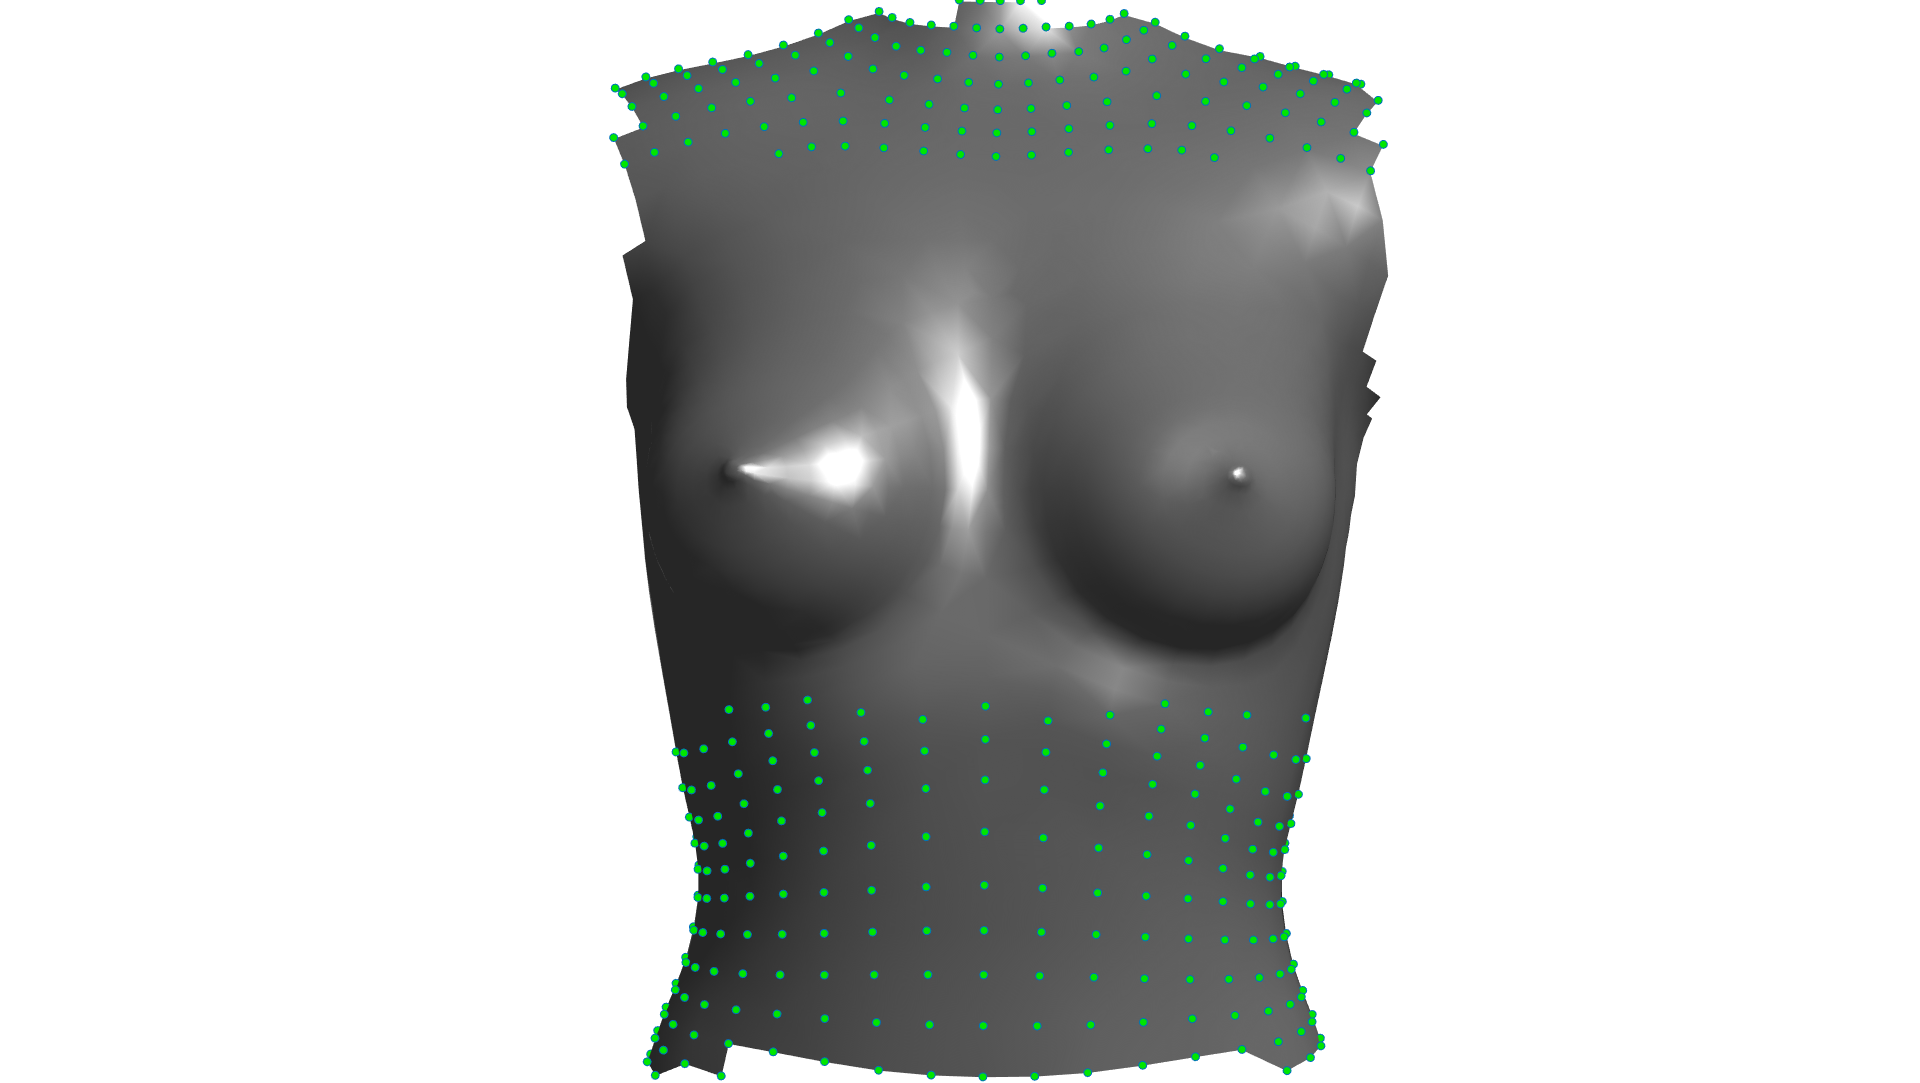
\includegraphics[width=0.75\textwidth]{figures/alignment}
\caption[Alignment points visualized]{The mesh is depicted as the grey surface. The green points are used for the alignment.}
\label{fig:alignment}
\end{figure}

\section{Parametric Model from Meshes}
In the next section, it is described how a parametric model is obtained using principle component analysis (PCA). This first method is the standard method, that is used in this thesis. In the following subsections, two different variations are described.
\subsection{Points}
\label{paramModel}
In this subsection, the general procedure to create a parametric model based on points, is described. Given $n$ meshes $m_i \in \mathbb{R}^{k \times 3}$, where $k$ describes the amount of vertices $m$ has, each mesh needs to be transformed to be of shape $\mathbb{R}^{1 \times 3k}$. Then, all transformed meshes are stacked into a matrix $M \in \mathbb{R}^{n \times 3k}$. As the differences over each column isn't significant, the mean $\bar{m}$ of the matrix $M$ is subtracted from each row of $M$.
\begin{gather}
\mathbf{A} :=
\begin{bmatrix}
 m_1' - \bar{m} \\
 m_2' - \bar{m} \\
 \vdots \\
 m_n' - \bar{m}
\end{bmatrix}
\in \mathbb{R}^{n \times 3k}
\end{gather}

Next, PCA is run with matrix $A$ as the input. PCA is able to reduce the dimensionality of the data, while retaining most of the information from the initial data set. This is achieved, by finding orthogonal basis vectors, where the first basis vector is responsible for the largest variance in the data. The second basis vector needs to be orthogonal to the first and is responsible for the second largest variance of the data. This holds for each following basis vector. These basis vectors in PCA are also known as principle components.

The output of the PCA function is:

\begin{gather}
\mathbf{coeff} :=
\begin{bmatrix}
 c_1&c_2&\cdots&c_{n-1}
\end{bmatrix}
\in \mathbb{R}^{3k \times n-1}
\end{gather}
\begin{gather}
\mathbf{score} :=
\begin{bmatrix}
s_1&s_2&\cdots&s_{n-1}
\end{bmatrix}
\in \mathbb{R}^{n \times n-1}
\end{gather}

where coefficient $c_i$ is the $i$-th principle component and score $s_i$ is the $i$-th parameter vector corresponding to the $i$-th input. Therefore, the input data can be reproduced by computing $\mathbf{A = score \times {coeff}^T}$. Instead of using all $n-1$ coefficients, it is possible to only use the first $\mathbf{q}$ coefficients resulting in an approximation of the space. The parameters $\mathbf{p_{q,new}}$ for a new input mesh $m_{new}$ can be easily computed for $\mathbf{q}$ coefficients, by first reshaping the mesh to be of the form $\mathbb{R}^{3k \times 1}$ and subtracting the mean $\bar{m}$. This is done the same way as above, adding an additional step to transpose. Then, the pseudoinverse of $\mathbf{coeff_{(q)}}$ is multiplied from the left to compute the corresponding parameters $\mathbf{p_{q,new}}$:
\begin{gather}
\mathbf{p_{q,new}} = \mathbf{coeff^+_{(q)}} \cdot (m_{new}' - \bar{m})^T  \text{  where }
\mathbf{coeff_{(q)}} :=
\begin{bmatrix}
 c_1&c_2&\cdots&c_{q}
\end{bmatrix}
\in \mathbb{R}^{3k \times q}
\end{gather}
The number of principle components used to approximate the space was reduced to $30$ in this thesis. In this example, the parametric model is based on the vertices of the mesh. In the next subsections, two other variants are explored and explained.
\subsection{Face Deformations}
\label{faceDeform}
Instead of defining a mesh by its vertices, it is possible to describe the mesh by the deformations of the faces. This is done by defining one source mesh and computing how each face is deformed in relation to the source mesh. One way to quantify a deformation of a face, was described by Sumner \cite{sumner2004deformation}, where the idea was to transfer triangle deformations between similar meshes. First, a new vertex needs to be computed, such that an affine transformation can be determined. The fourth vertex is defined as follows:
\begin{gather}
  \mathbf{v_4} = \mathbf{v_1} + (\mathbf{v_2} - \mathbf{v_1})\cross(\mathbf{v_3}-\mathbf{v_1})/\sqrt{\lvert(\mathbf{v_2}-\mathbf{v_1})\cross(\mathbf{v_3}-\mathbf{v_1})\rvert} \label{normalequation}
\end{gather}

\begin{figure}[h]
\centering
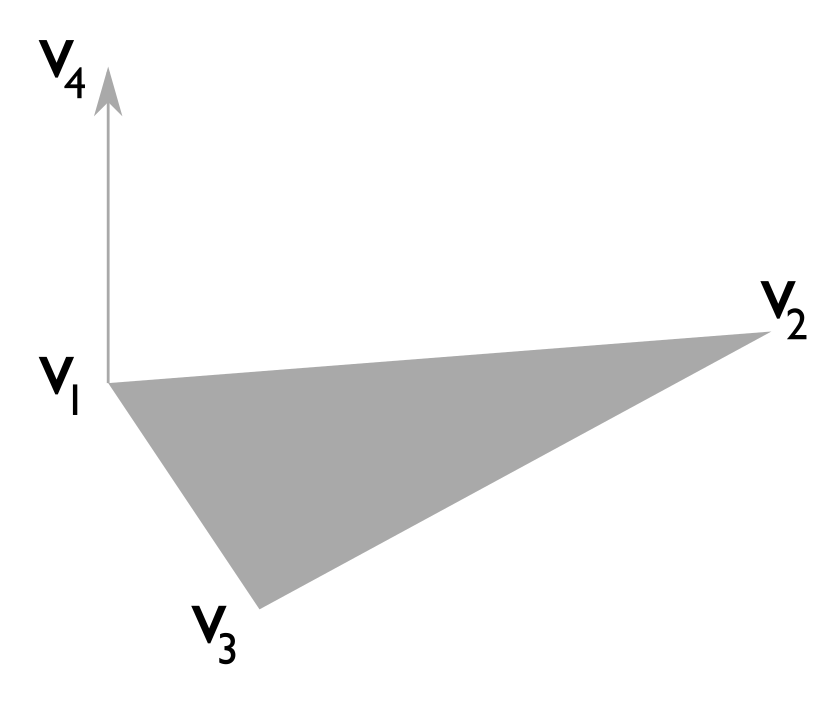
\includegraphics[width=0.4\textwidth]{figures/normal}
\caption[Diagram point on normal]{A vertex is added to the triangle that lies in the direction of the normal.}
\label{fig:normal}
\end{figure}

The cross product is scaled by the reciprocal of the square root of its length, to keep the distance proportional to the length of the triangle edges. See figure \ref{fig:normal} for a visualization of adding a vertex on the normal.
Given both triangles with one additional vertex, the following equations can be posed:
\begin{gather}
 \mathbf{Q}\mathbf{v_i}+\mathbf{d} = \mathbf{\tilde{v}_i}, \mathbf{i} \in \mathbf{1} \dotsc \mathbf{4}
\end{gather}
where $\mathbf{Q} \in \mathbb{R}^{3 \cross 3}$ and translation vector $\mathbf{d}$ describe the affine transformation. By subtracting the first equation from the following three equations and rewriting the resulting system in matrix form, the problem can be defined as $\mathbf{Q}\mathbf{V}=\mathbf{\tilde{V}}$ where
\begin{gather}
  \mathbf{V} =
  \begin{bmatrix}
   \mathbf{v_2} - \mathbf{v_1}&\mathbf{v_2} - \mathbf{v_1}&\mathbf{v_2} - \mathbf{v_1}
  \end{bmatrix} \\
  \mathbf{\tilde{V}} =
  \begin{bmatrix}
   \mathbf{\mathbf{v}_2} - \mathbf{\mathbf{v}_1}&\mathbf{\mathbf{v}_2} - \mathbf{\mathbf{v}_1}&\mathbf{\mathbf{v}_2} - \mathbf{\mathbf{v}_1}
  \end{bmatrix}
\end{gather}
The closed form expression for $\mathbf{Q}$ is defined as
\begin{gather}
  \mathbf{Q}=\mathbf{\tilde{V}}\mathbf{V}^{-1}
\end{gather}
To fully describe a mesh, this $\mathbf{Q}$ matrix needs to be computed for each face of the mesh. Finally, the mesh is represented by $\mathbf{D} \in \mathbb{R}^{3 \times 3h}$ where $\mathbf{h}$ is the number of triangles the mesh has. To be able to run PCA, each mesh needs to be reshaped to be of form $\mathbf{D'} \in \mathbb{R}^{1 \times 9h}$ and the rest of the process is the same as above in section \ref{paramModel}.

\subsection{Point Normals}
This method is very much similar to the one described in section \ref{paramModel}. In addition to the vertices of the mesh, one vertex per face is computed as described in equation \ref{normalequation} and added to the list of vertices of the mesh. Therefore, the mesh matrix will be of form $\mathbb{R}^{k+h \times 3}$, where $\mathbf{k}$ is the number of original vertices and $\mathbf{h}$ is the number of triangles of the mesh.

\section{Mapping}
The following segment describes how a mapping can be computed in a linear or a non-linear way. The data available is the parameters returned by both the parametric models for the \textit{before} and \textit{after} examples. The matrices of the data are
\begin{gather}
  \mathbf{P_{before}} =
  \begin{bmatrix}
    \mathbf{p_{b,1}} \\
    \mathbf{p_{b,2}}  \\
    \vdots \\
    \mathbf{p_{b,n}}
  \end{bmatrix}
  \in \mathbb{R}^{n \cross n-1},
  \mathbf{P_{after}} =
  \begin{bmatrix}
    \mathbf{p_{a,1}} \\
    \mathbf{p_{a,2}} \\
    \vdots \\
    \mathbf{p_{a,n}}
  \end{bmatrix}
  \in \mathbb{R}^{n \cross n-1}
\end{gather}
where each parameter pair $(\mathbf{p_{b,i}}, \mathbf{p_{a,i}})\ \forall i$ is related, as the \textit{after} was generated from the \textit{before}.

\subsection{Linear Method}
The first method used, was the linear system solver by MATLAB (also known as backslash \ solver) that solved the equation
\begin{gather}
  \mathbf{P_{before}} \cdot \mathbf{M_{linear}} = \mathbf{P_{after}}
  \text{ where } M_{linear} \in \mathbb{R}^{n-1 \times n-1}.
\end{gather}
It is clear, that an explicit linear transformation could be found for each parameter pair, but the goal is to have one mapping that works for each parameter pair. This is also known as linear regression. One basic example in linear regression is the task of fitting a line to a point cloud. As all the points of the point cloud do not lie on one line, it isn't possible to define a straight line. Therefore, a line is sought after, such that all points are as close as possible on average. This is depicted in figure \ref{fig:linReg}.

\begin{figure}[h]
\centering
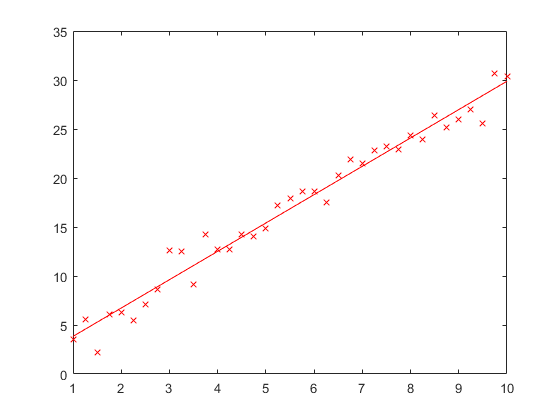
\includegraphics[width=0.7\textwidth]{figures/linReg}
\caption{Fitting a line to a point cloud using linear least-squares.}
\label{fig:linReg}
\end{figure}

\subsection{Non-Linear Variants}
\label{sec:nonLin}
This section deals with non-linear methods to solve the regression problem described above. All the methods used are part of the scikit-learn library \cite{scikit-learn}. It is common in a machine learning setting to split data into two sets. One set is used to train the model and the other is used to evaluate how well the method does on data, that was not part of the first set. Both data sets should be drawn from the same distribution. This is necessary because the model shouldn't be penalized for performing badly on problems it didn't encounter in the training phase.\\
During the training phase, it is standard to run grid search. Grid search varies the parameters of the model to find the best set of parameters for a specific task. It needs to be considered, that grid search can lead to overfitting. This occurs when the error on the training set is reduced at the cost of increasing the test error. This can be avoided by adding regularization terms or by running grid search along with cross-validation.
\subsubsection{Decision Tree}
\label{sec:dt}
One category of machine learning approaches is based on so called decision trees (DT). A decision tree uses a tree-like approach, where nodes of the tree are defined to split the data set into subsets corresponding to groups. As an example, the goal is to have a model that can predict the weight of a person, based on height, daily activity and daily calorie intake as features. Using a decision tree, the value of height could split the data set, as taller people tend to be heavier than small people. This is done over all features until the complete data set is divided into smaller subsets. Leafs make up the end of a decision tree. Each leaf has a certain value connected to it, in the case mentioned before it would be a certain weight range or value. \\
When the weight of a new person would need to be predicted, one would follow the tree from top to bottom until a leaf was met. The corresponding weight value of the leaf would be equal to the prediction the model returns. An example of a decision tree can be seen in figure \ref{fig:dtdiag}.

\begin{figure}[h]
\centering
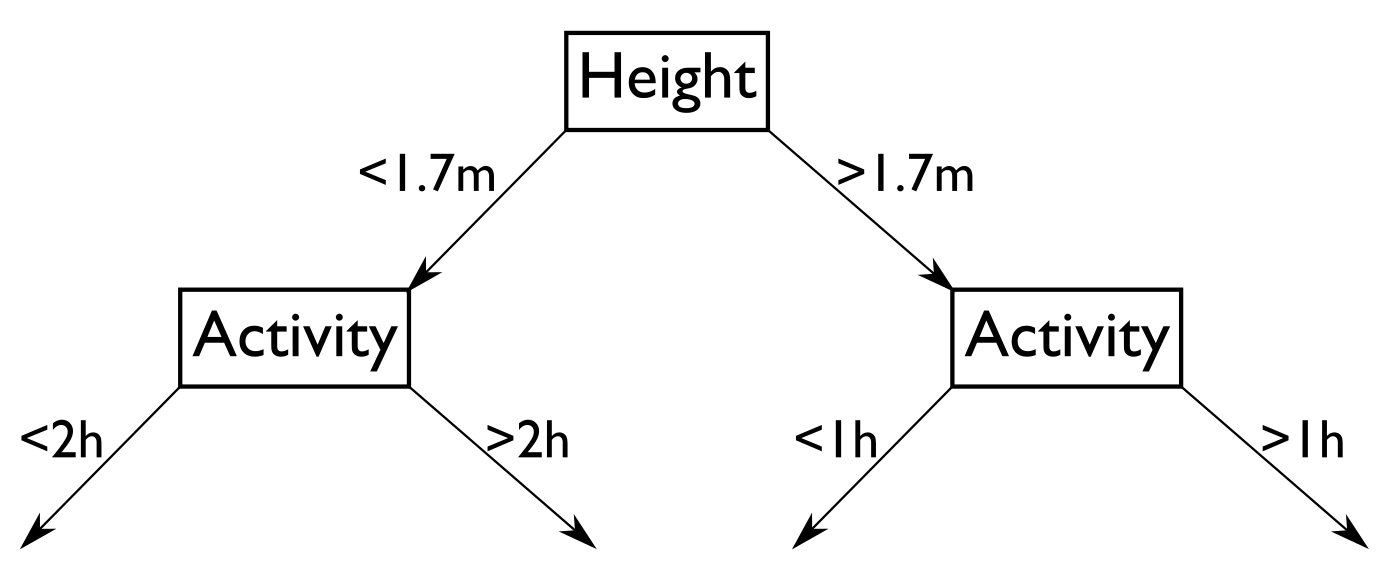
\includegraphics[width=0.75\textwidth]{figures/dtdiag}
\caption[Diagram of decision tree]{Example of a decision tree following example of section \ref{sec:dt}}
\label{fig:dtdiag}
\end{figure}

\newpage

\subsubsection{Random Forest}
The random forest (RF) regressor is also a tree-like approach, similar to the decision tree. The main difference is, that the decision tree considers all features when splitting and thus can be prone to overfitting. Random forest chooses features at random and builds decision trees based on those features. This is done for multiple trees until all subtrees are combined.

\subsubsection{Multilayer Perceptron}
The multilayer perceptron (MLP) is a type of neural network. It uses a feedforward approach to propagate information through the network. MLP has at least three layers, where the first layer is the input layer and the last layer is the output layer. Each layer is made up of neurons, that receive information from the previous layer, apply a multiplication with a weight and an addition of a bias term followed by an activation function and pass the result on to the next layer. These activations can either be linear or non-linear. It doesn't make sense to have multiple intermediate layers with linear activation functions, as any combination of linear functions can be described by one linear function. \\
Each layer is made up of multiple neurons, each with their own weights and biases, and an activation function. All weights and biases are initialized at random. In the training phase, a technique known as backpropagation is applied. Given an example, input and outcome, the input data is passed through all the layers. The resulting output is compared to the actual outcome. Given the difference between the two values, weights and biases are modified to reduce the difference, starting from the output layer, moving back through the hidden layers, up to the input layer. A basic scheme of a MLP is shown in figure \ref{fig:mlpdiag}.

\begin{figure}[h]
\centering
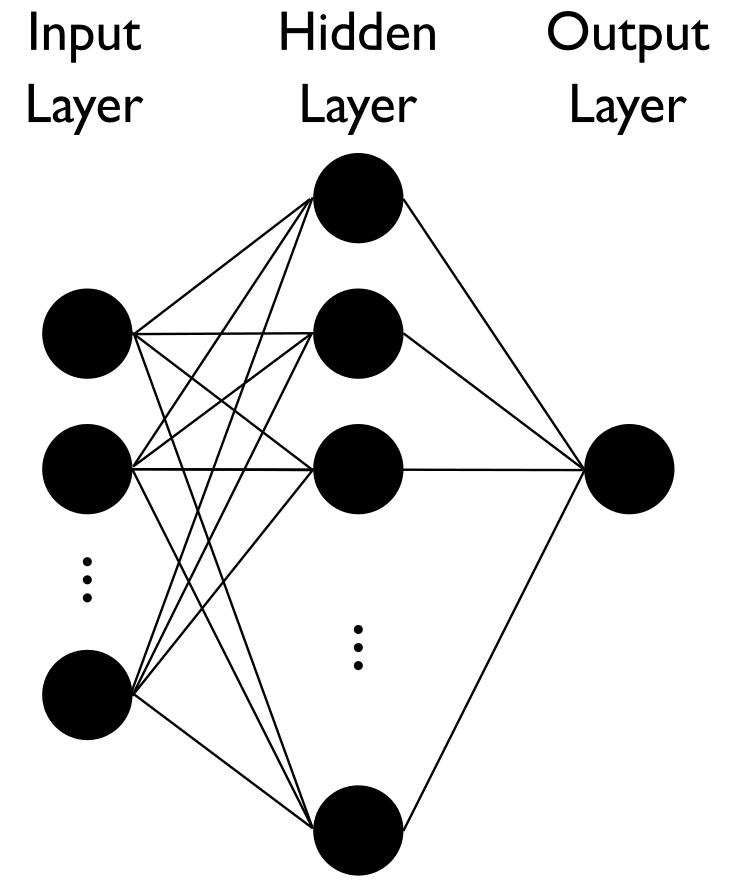
\includegraphics[width=0.3\textwidth]{figures/mlpdiag}
\caption{Scheme of a multilayer perceptron for regression.}
\label{fig:mlpdiag}
\end{figure}


\section{Parametric Model from Editor}
In all of the previous sections, the parametric model was based off of real world data. In this section, the same procedure is done as in section \ref{paramModel}, except that the meshes used for PCA were generated by software called MakeHuman \footnote{http://www.makehumancommunity.org/}. MakeHuman is a free and open source character modelling tool. It starts out with a gender neutral base mesh that can be modelled by varying sliders. These sliders apply linear interpolations to the base mesh between the extreme positions for a specific semantic parameter.\\
There are over 40 semantic parameters in MakeHuman and the semantic parameters are categorized by what areas of the body they modify. The graphical user interface of MakeHuman can be seen in figure \ref{fig:mhgui}. Using the scripting feature in MakeHuman, multiple meshes could be generated, exported and later imported into MATLAB.

\begin{figure}[h]
\centering
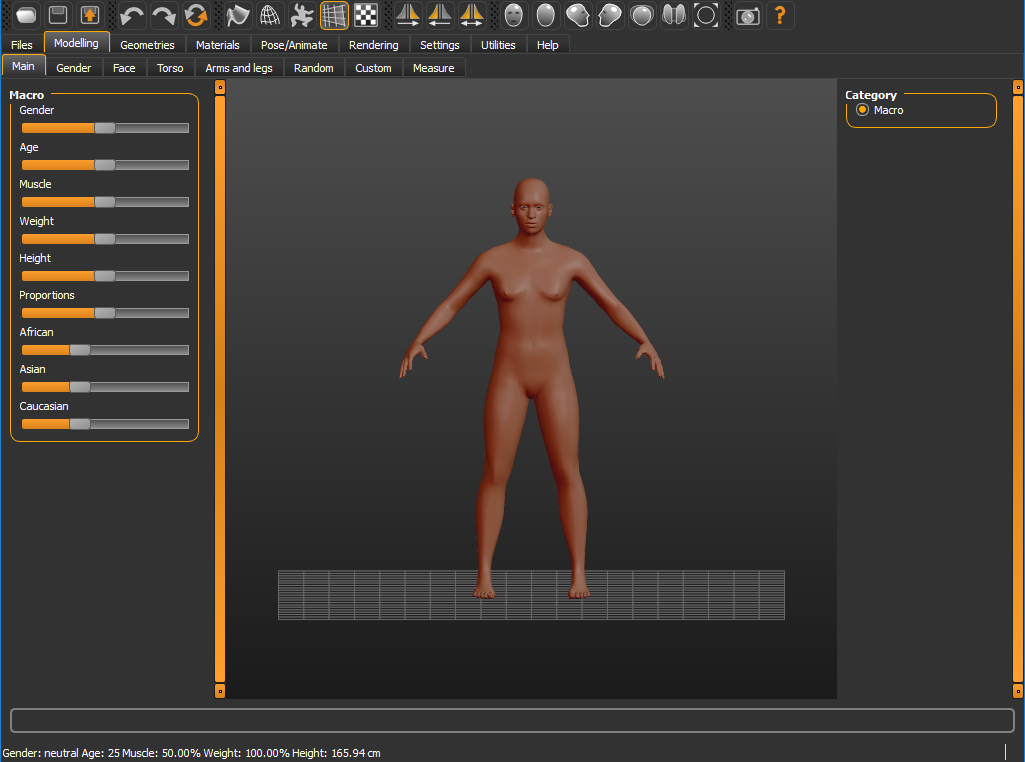
\includegraphics[width=1\textwidth]{figures/mhgui}
\caption[MakeHuman interface]{Graphical user interface of MakeHuman. On the left some of the semantic parameters can be seen.}
\label{fig:mhgui}
\end{figure}

\section{Fitting parametric models to point clouds}
\label{fitModel}
Given a parametric model, it is possible to create a large diversity of possible outputs by varying the parameters. But finding the specific parameters for a new point cloud is a non-linear optimization problem. Therefore, a C++ implementation by Biland \cite{Biland17}, using an open source C++ library for optimization problems called the Ceres solver \cite{ceres-solver}, was slightly modified and used. This implementation allows to fit a parametric model to a point cloud given a few keypoints of the point cloud. The slight modification enables a list of indices to be used as candidates for the correspondences required.\\
In a first step, the keypoints are used to find the parameters of translation, rotation and scaling. Afterwards, a select number of points are chosen as correspondences for the model and, using a nearest neighbour approach, the closest points in the point cloud are found. This implementation tries to minimize the distance between all the correspondences iteratively, by varying the parameters of the model. Additionally, constraints are applied to the values the parameters are allowed to take. This prevents one parameter from becoming too large and also possibly forces the model to use multiple parameters rather than to rely on a single parameter. After a certain number of iterations has been reached, a certain threshold in accuracy is passed or the change in parameters is vanishingly small, the resulting mesh and parameters are returned.

\chapter{Results}
In the next section, two error metrics are briefly described, followed by evaluations of each experiment. At the beginning of each section a small description of the problem setting is given, followed by the results and discussion.

\section{Error Metrics}
\label{Emetrics}
For this thesis two error metrics were considered:
\begin{itemize}
  \item \textbf{Point Distance:} Given two meshes with equal topology, meaning both meshes have the same amount of vertices and layout, the error computed is based on the distance between corresponding points. In general, the mean distance is computed over all point correspondences.
  \item \textbf{Face orientations:} The idea behind this method is based on the $\mathbf{Q}$ matrix mentioned in section \ref{faceDeform}. Given two topologically equal meshes, the $\mathbf{Q}$ matrix is computed for all corresponding triangles. As it is of interest to investigate the difference in breast shapes, this error tries to quantify the variation of the $\mathbf{Q}$ matrices.
\end{itemize}

One drawback of the point distance method occurs, when the two meshes are not aligned properly. This can be solved by applying the same algorithm mentioned in section \ref{align} before computing the error. One advantage of this method is the unit of the error, as it could be converted into a unit of distance, given that the distance between two points is known in real world lengths. This error can also be computed, when two meshes are not topologically equal, by first finding the correspondences between vertices.\\
One advantage of the face orientation method is the invariance of translation and global rotation. This means, that moving or rotating the mesh doesn't affect the error. On the other hand, the values of this error don't have a real world meaning and it is a lot harder to apply this method to topologically different meshes, as finding correspondences between triangles is a lot more challenging.\\
The methods are depicted in figure \ref{fig:errordiag}. Both methods have their advantages and disadvantages, but due to the fact that alignment isn't a problem, the error metric used in this thesis is the point distance method. Additionally, based on the MakeHuman model, the distance between the belly button and throat is approximated to be $40.6cm$. This is taken as an assuption for both meshes, such that all distances can be computed in centimetres.

\begin{figure}
\centering
\begin{subfigure}{.5\textwidth}
  \centering
  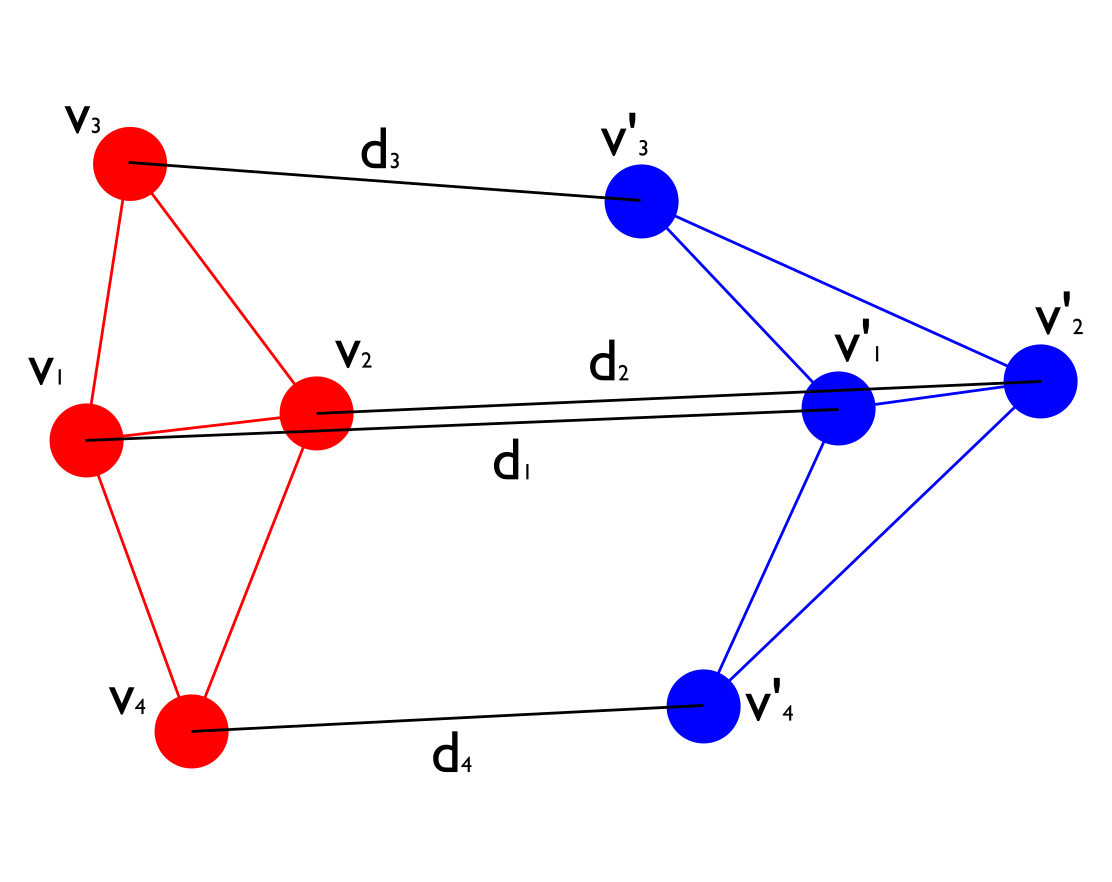
\includegraphics[width=.75\linewidth]{figures/pediag}
\end{subfigure}%
\begin{subfigure}{.5\textwidth}
  \centering
  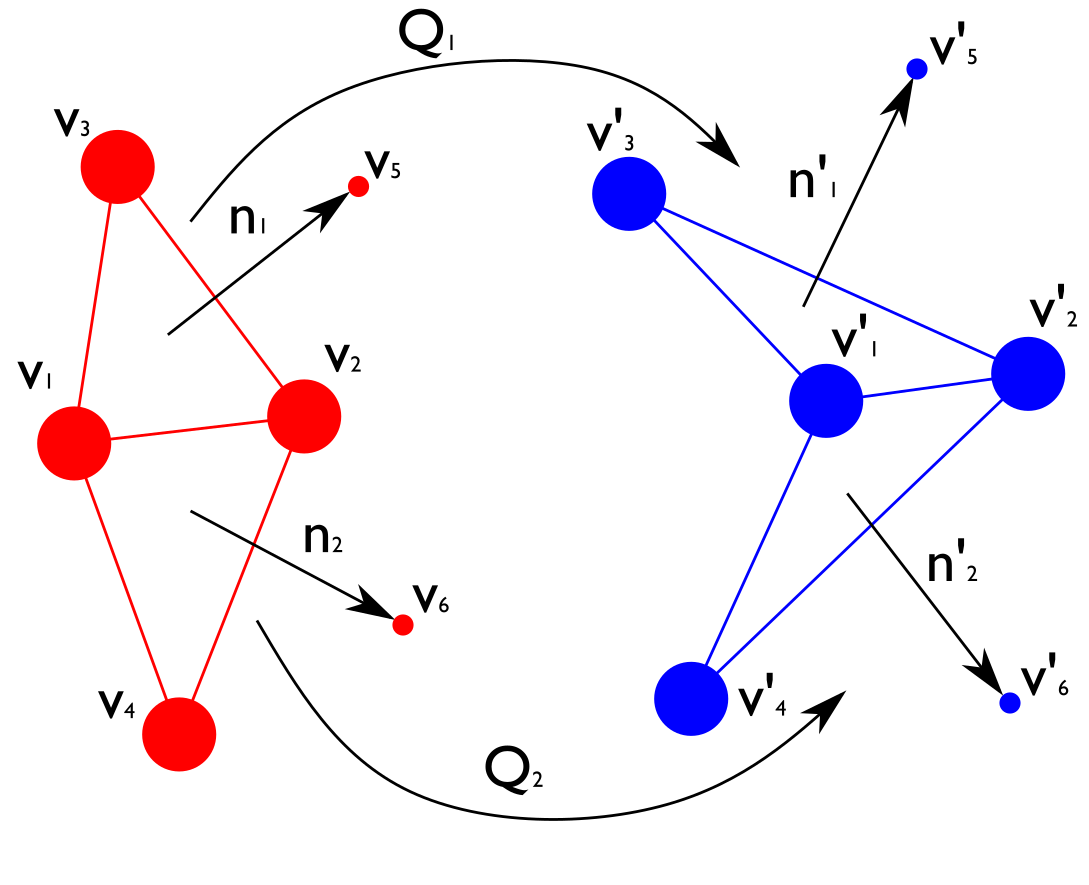
\includegraphics[width=.75\linewidth]{figures/dediag}
\end{subfigure}
\caption[Error metric diagrams]{The left image depicts distances between corresponding points of the mesh. The right image shows a representation of the information used to compute the $\mathbf{Q}$ matrix.}
\label{fig:errordiag}
\end{figure}

\section{Evaluation}
In the following section, the evaluation methods that were used are explained. Optimally, when evaluating a prediction, some representation of the true outcome, often called the "ground truth", is given. This is useful to quantify how accurate the prediction was.
\subsection{Mesh Point Error} % Compare to GT
\label{mpError}
For this method the comparison is done as explained in section \ref{Emetrics}. Before evaluating the point distances between a prediction and the ground truth, the meshes are aligned, as mentioned in section \ref{align}. Additionally, the mean point distance error is computed by dividing by the number of vertices in the mesh and also by multiplying with the approximated centimetre length of one unit in mesh space. This allows to transform all values into centimetres. Given a prediction of a mesh $M^{(p)}$ and the ground truth $M^{(g)}$ the problem can be stated as:
\begin{gather}
error = s_{cm}\sum_{i=1}^{n} \sqrt{\sum_{j=1}^3(M_{i,j}^{(p)} - M_{i,j}^{(g)})^2}
\end{gather}
where $n$ is the number of vertices of the mesh, $s_{cm}$ is the approximated length in centimetres equivalent to one unit distance in mesh space.
\subsection{Error Heat Map} % Compare to NRICP vs Ceres
\label{mhError}
The idea of this method, is to generate a visualization of the error, indicating where the prediction failed to represent the ground truth the most. This can be accomplished by computing the error described in section \ref{Emetrics}, but instead of adding up the errors per mesh, the errors are stored separately for each vertex. This error per vertex is accumulated over multiple samples and the mean is computed. Given the k-th prediction of a mesh $M^{(p_k)}$ and the corresponding ground truth $M^{(g_k)}$ the problem can be described as:
\begin{gather}
e'_{i} = \frac{s_{cm}}{m} \sum_{k=1}^{m} \sqrt{\sum_{j=1}^3(M_{i,j}^{(p_k)} - M_{i,j}^{(g_k)})^2} \  \forall i=1 \dots n \text{ with } e = \frac{e'}{max(e')}
\end{gather}
where $m$ is the number of samples, $s_{cm}$ is the approximated length in centimetres equivalent to one unit distance in mesh space, $e'$ is a vector of the accumulated errors over all samples and $e$ is a vector of the errors scaled inversely by the largest entry in $e'$. This is done to visualize the error on a range, such that, for example, the error can be color coded, where dark red is equivalent to a large error and blue is a small error.

\section{Input Data for PCA}
In this experiment, three different variations of data inputs are tested for PCA, as described in section \ref{paramModel} and the following two subsections. Based on the resulting parameters of each model, a linear mapping is created and compared based on the error of the predictions.

\subsection{Problem Setting}
Given a data set comprised of 57 pairs of meshes, where one mesh is based on the \textit{before} point cloud and the other is based on the \textit{after} point cloud, both sets are split into equally-sized sets of 42 training pairs and 15 testing pairs. Each variation is trained on the training set and afterwards evaluated on the test set. The evaluation is done by computing a linear mapping over the parameters of each model. Then, the mean mesh point error over all 15 testing pairs is computed and an error heat map is generated.
\subsection{Results}
In the table \ref{tablePDN}, the time column is the amount of time each method needed to compute the parametric model. The training mean error is computed as mentioned in \ref{mpError} for each case. The mean is computed over all cases. The same is done for the test mean error. The errors for the error heat maps were computed on the test set. In each subfigure of figure \ref{fig:PDNheatmap} the values that are listed above are the respective $\mathbf{max(e')}$, as explained in \ref{mhError}. Additionally, one vertex on the border doesn't have a colored point, as the error wasn't being computed correctly for it.

\begin{table}[]
\centering
\begin{tabular}{l|l|l|l|l|}
\cline{2-5}
                                                  & \textbf{Time (s)} & \textbf{\begin{tabular}[c]{@{}l@{}}Training\\ Mean Error (cm)\end{tabular}} & \multicolumn{2}{l|}{\textbf{\begin{tabular}[c]{@{}l@{}}Test\\ Mean Error (cm)\end{tabular}}} \\ \hline
\multicolumn{1}{|l|}{\textbf{Point}}              & 0.06         & 0.40                                                                & \multicolumn{2}{l|}{1.01}                                                            \\ \hline
\multicolumn{1}{|l|}{\textbf{Deformation}}        & 6.81         & 0.49                                                                 & \multicolumn{2}{l|}{1.53}                                                            \\ \hline
\multicolumn{1}{|l|}{\textbf{Points and Normals}} & 2.92         & 0.39                                                                 & \multicolumn{2}{l|}{1.01}                                                            \\ \hline
\end{tabular}
\caption[Table of results of Input Data for PCA]{Results in terms of mean mesh point error are listed for the training and for the test set in centimetres. Additionally, the time each function took to compute the parametric model is listed in seconds.}
\label{tablePDN}
\end{table}

\begin{figure}
\centering
\makebox[\textwidth][c]{%
  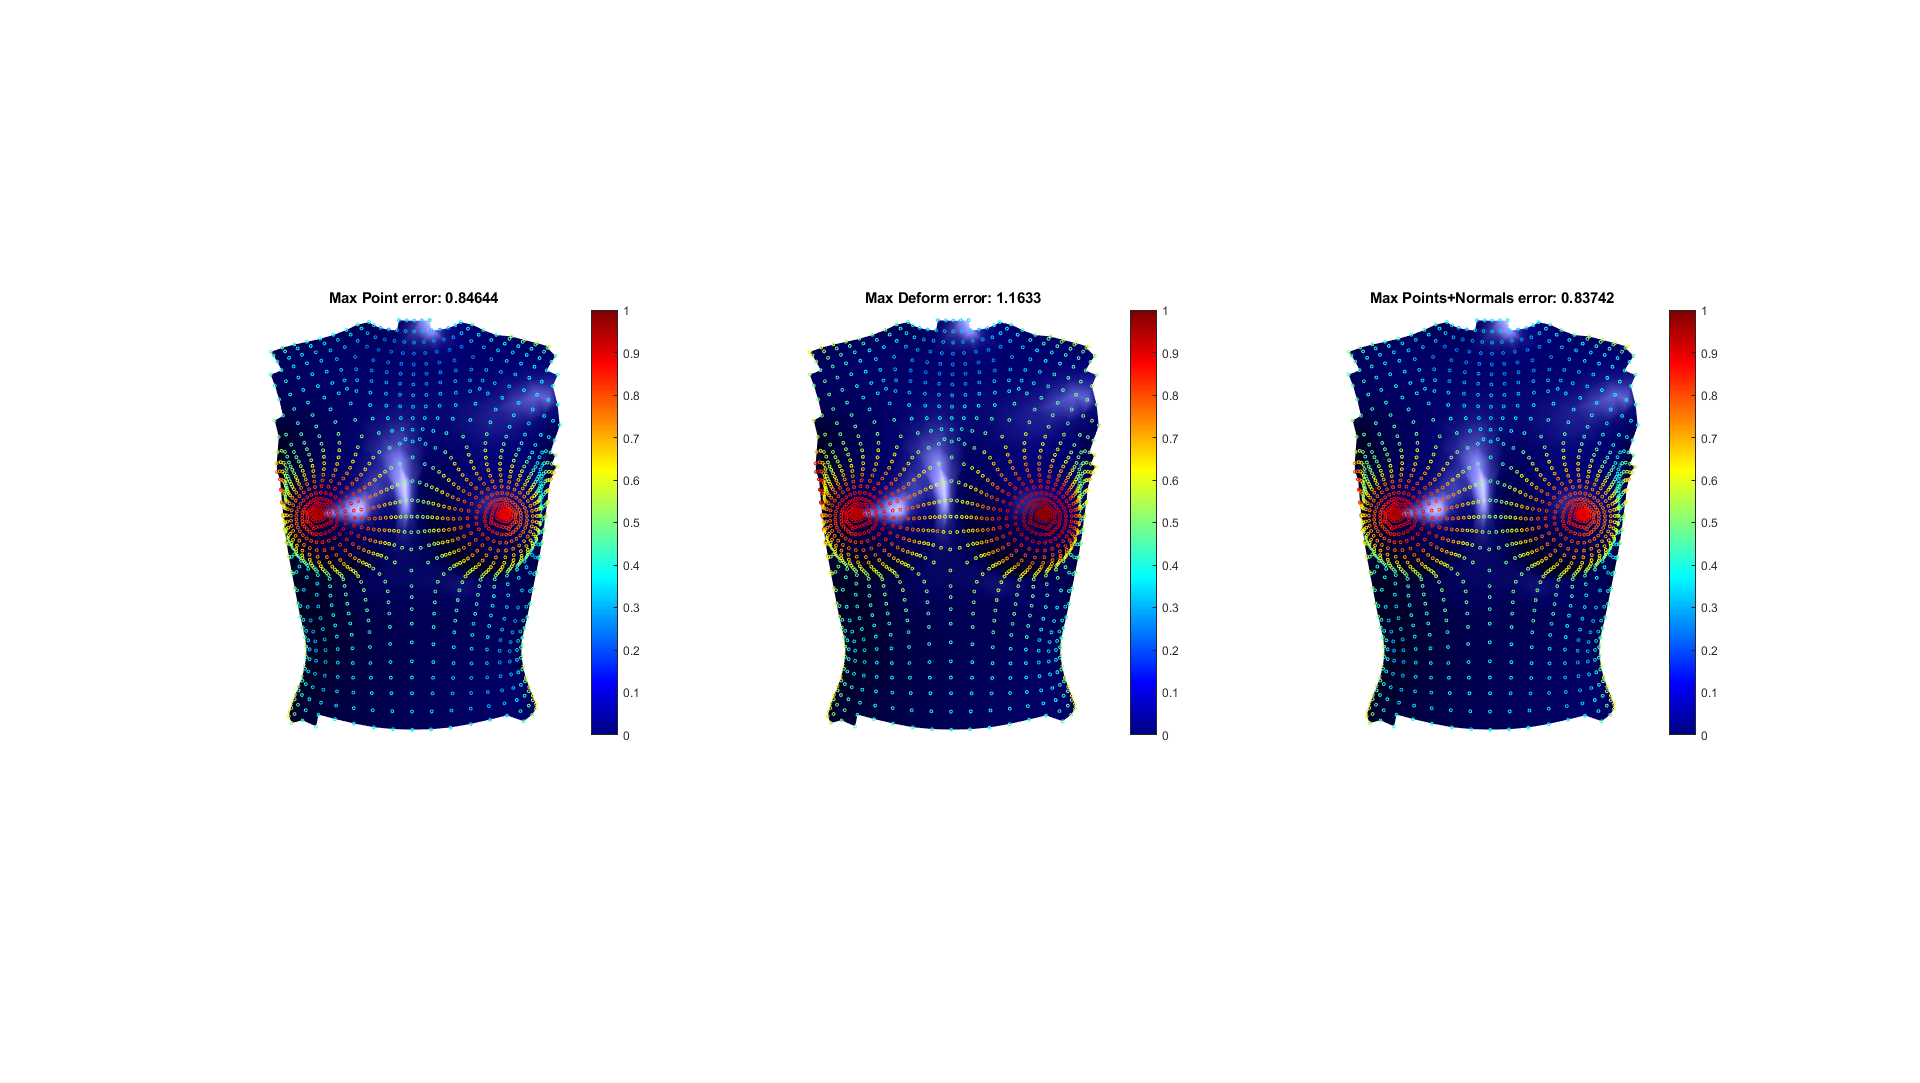
\includegraphics[width=1.6\textwidth]{figures/evalPDN}%
}
\caption[Input Data for PCA error heat map]{The left image shows the error heat map when using the points method. The middle one uses the deformation method. The right one uses the point normals method. The color of each point reflects the amount of the error. Red color indicates large error, blue small error.}
\label{fig:PDNheatmap}
\end{figure}

\subsection{Discussion}
The amount of time it takes to compute the parametric model, based on deformations, is much larger. This is due to the fact, that additional points on the normals of each triangle need to be computed, followed by computations of the $Q$ matrix for each triangle. One can see, that the additional time to compute normals is also reflected in the point and normals method. Therefore, roughly $\mathbf{40\%}$ of the time is accounted for by the normal computation. The points method is by far the fastest method.\\
All three methods worsen going from training to test sets in terms of error, but that is expected. This is caused by the models having seen the training set before and are already familiar with those examples. Of the three methods, the point and normals method achieves the best results over test and training. The reason this occurs is due to the fact, that the normals carry information of the size of the triangles.\\
Figure \ref{fig:PDNheatmap} looks similar for all three cases. The error for the deformation method is higher than for the other two methods. This might be caused by the deformation method performing well in terms of triangle orientation, at the cost of some vertices being displaced. Around the right breast, the red area seems larger and darker than for the other two methods. The deformation method might have more difficulty placing the nipple correctly. Visually, no difference can be made out between the points method and the point normals method,

\section{Learning Mapping}
The next step was to investigate, if non-linear mappings could perform better than a linear mapping. Additionally, it is analyzed how the error behaves, when PCA is done on the complete set, instead of only the training set. The reason this is done, is because the mapping shouldn't be penalized or perform badly because of the parametric model. For each of the approaches, the best parameters need to be found first by running cross-validation grid search. Each of the learnt mappings can be applied to the test set and compared against the ground truth. The mean point error is computed to measure the error.

\subsection{Problem Setting}
The parameters for each of the 57 pair meshes are computed according to two parametric models. These will be referred to as the "complete" and "incomplete" model, where the "complete" model was based on the training and test data, whereas the "incomplete" model only received the training data. The non-linear approaches used, are a decision tree regressor, a random forest regressor, a multilayer perceptron with a rectified linear unit (ReLU) as its activation function and a multilayer perceptron with any other activation function except a ReLU. \\
For each approach the best parameters are evaluated by running 6-fold cross-validation grid search for either cases, where the error is not minimized in parameter space, but in mesh space. The method's varied parameters are listed in a table, that can be found in the appendix \ref{gstable}. Finally, the training and test errors are computed based on the best parameters and a ratio between test and training error is calculated. Optimally, this ratio should be one, as the test error should be equally low as the training error.

\subsection{Results}
The results for the different cases can be seen in \ref{tableMapping}. The table is divided into two sections, the first half for the results of the "incomplete" model and the second for the "complete" model. The first row of results are the mean errors for the training set, the second row for the test set. The error for a prediction is computed by comparing to the ground truth with the mesh point error, as explained in \ref{mpError}. The resulting error is equivalent to the mean over all errors. The last column is the ratio between test and training error.

\begin{table}[]
\centering
\begin{tabular}{l|l|l|l|l|}
\cline{2-5}
\textbf{PCA Model}  & \textbf{Method}        & \textbf{\begin{tabular}[c]{@{}l@{}}Training\\ Mean Error (cm)\end{tabular}} & \textbf{\begin{tabular}[c]{@{}l@{}}Test\\ Mean Error (cm)\end{tabular}} & \textbf{\begin{tabular}[c]{@{}l@{}}Ratio\\ Test/Train\end{tabular}} \\ \cline{2-5}
\textbf{Incomplete} & \textbf{Linear}        & 0.40                                                                 & 1.01                                                             & 2.52                                                                \\ \cline{2-5}
\textbf{}           & \textbf{Random Forest} & 0.37                                                                 & 1.07                                                             & 2.88                                                                \\ \cline{2-5}
\textbf{}           & \textbf{Decision Tree} & 0.69                                                                 & 1.30                                                             & 1.86                                                                \\ \cline{2-5}
\textbf{}           & \textbf{MLP}           & 0.84                                                                 & 1.02                                                             & 1.21                                                                \\ \cline{2-5}
\textbf{}           & \textbf{MLP ReLU}      & 0.95                                                                 & 1.11                                                             & 1.17                                                                \\ \cline{2-5}
\textbf{Complete}   & \textbf{Linear}        & 0.42                                                                 & 1.95                                                             & 4.70                                                                \\ \cline{2-5}
\textbf{}           & \textbf{Random Forest} & 0.42                                                                 & 1.07                                                             & 2.55                                                                \\ \cline{2-5}
\textbf{}           & \textbf{Decision Tree} & 0.68                                                                 & 1.19                                                             & 1.74                                                                \\ \cline{2-5}
\textbf{}           & \textbf{MLP}           & 0.83                                                                 & 1.06                                                             & 1.27                                                                \\ \cline{2-5}
\textbf{}           & \textbf{MLP ReLU}      & 0.88                                                                 & 1.06                                                             & 1.20                                                                \\ \cline{2-5}
\end{tabular}
\caption[Learnt mapping results]{This tables shows the mean errors computed on the training and test set in centimetres. The first five rows show the results for the "incomplete" model, the last five for the "complete" model. The first two columns are the training and test error, followed by the ratio of test to training error.}
\label{tableMapping}
\end{table}

\subsection{Discussion}
It is interesting to see, that the training error of the linear method and the random forest increases slightly going from the "incomplete" to the "complete" model. This must be caused by some examples in the test set being similar to some of the examples in the training set and forcing the parameters to adjust. The other three methods improve slightly in terms of training error due to the "complete" model. Independant of case, the test error is always larger than the training error. This is expected and was already discussed above.\\

The behaviour of the test error going from "incomplete" to "complete" is similar to the training error. The linear method worsens gravely, perhaps due to the "complete" model describing a wider space, making it harder for the linear method to find an appropriate mapping. All of the non-linear methods perform similarly in the "complete" case compared to the "incomplete" case in terms of mean test error.\\

Even though the best performing method in terms of error is the MLP, the MLP with ReLU has similar error values but has a slightly better test/train ratio. This could indicate that this method is more robust, meaning that the expected error for new data should be similar. It can be seen, that all non-linear methods outperform the linear method. This difference in performance could increase drastically, when the model gets more complex due to more data.

\newpage

\section{Parametric Models}
For this experiment, it is explored how a parametric model based on an editor like MakeHuman performs against a model based on real data. As the topologies of the meshes used for the parametric models are different, the models are seperately evaluated and the resulting error heat maps are compared. Both models are tested, using the Ceres implementation by Biland \cite{Biland17}, mentioned in section \ref{fitModel}. The resulting mesh is then compared to the NRICP solution.

\subsection{Problem Setting}
Firstly, a parametric model is created from MakeHuman. To achieve this, 8 semantic parameters of the editor are varied between 3 positions and exported into MATLAB. The semantic parameters and values used can be found in the appendix in table \ref{tableSemantic}.
This results in 6'561 meshes, which are used to generate a parametric model. For the model based on real data, the parametric model generated from the \textit{before} meshes, is used. The ground truth meshes for the real data are already available, as those point clouds were already processed earlier. The ground truth meshes for the MakeHuman model are generated by running NRICP with a modified MakeHuman mesh. The difference between the original mesh and the modified MakeHuman mesh can be seen in figure \ref{fig:mhcut}.

\begin{figure}[h]
\centering
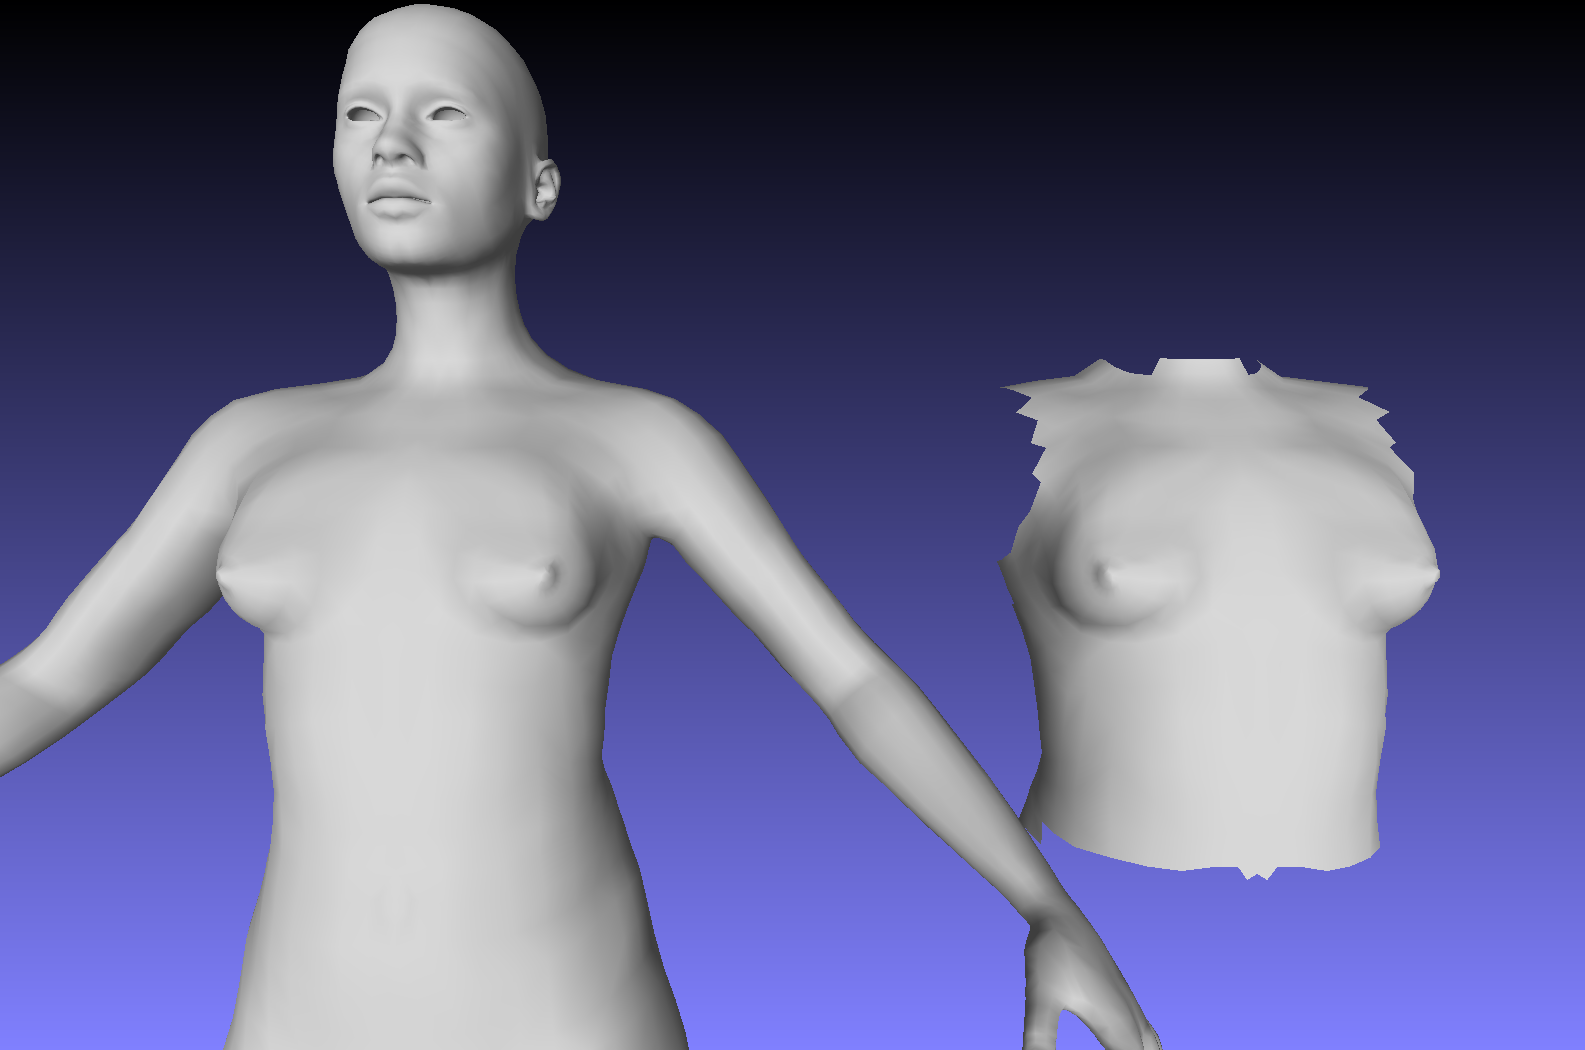
\includegraphics[width=0.5\textwidth]{figures/meshcut00}
\caption[Cut MakeHuman mesh]{On the left, the original mesh of MakeHuman can be seen. The cut mesh is on the right.}
\label{fig:mhcut}
\end{figure}

The Ceres implementation is run for both parameteric models, fitting both models to the test set of \textit{before} point clouds. The resulting meshes are then compared to the ground truth, by generating an error heat map for both models. The parameters used in the implementation can be found in the appendix in table \ref{tableCeresParams}.

\subsection{Results}
In figure \ref{fig:compparammodel}, the error in distance per vertex is accumulated over all test set examples. The maximum vertex error is stated above the mesh for each model respectively, left for MakeHuman and right for real data. All errors were scaled inversely by the largest error, coloring the largest errors dark red and small errors dark blue. For the MakeHuman model the largest errors arise around the nipple and the lower side of the breast. The real data model has the largest error around the nipple and the area to the outside of the breast.

\begin{figure}
\centering
\begin{subfigure}{.5\textwidth}
  \centering
  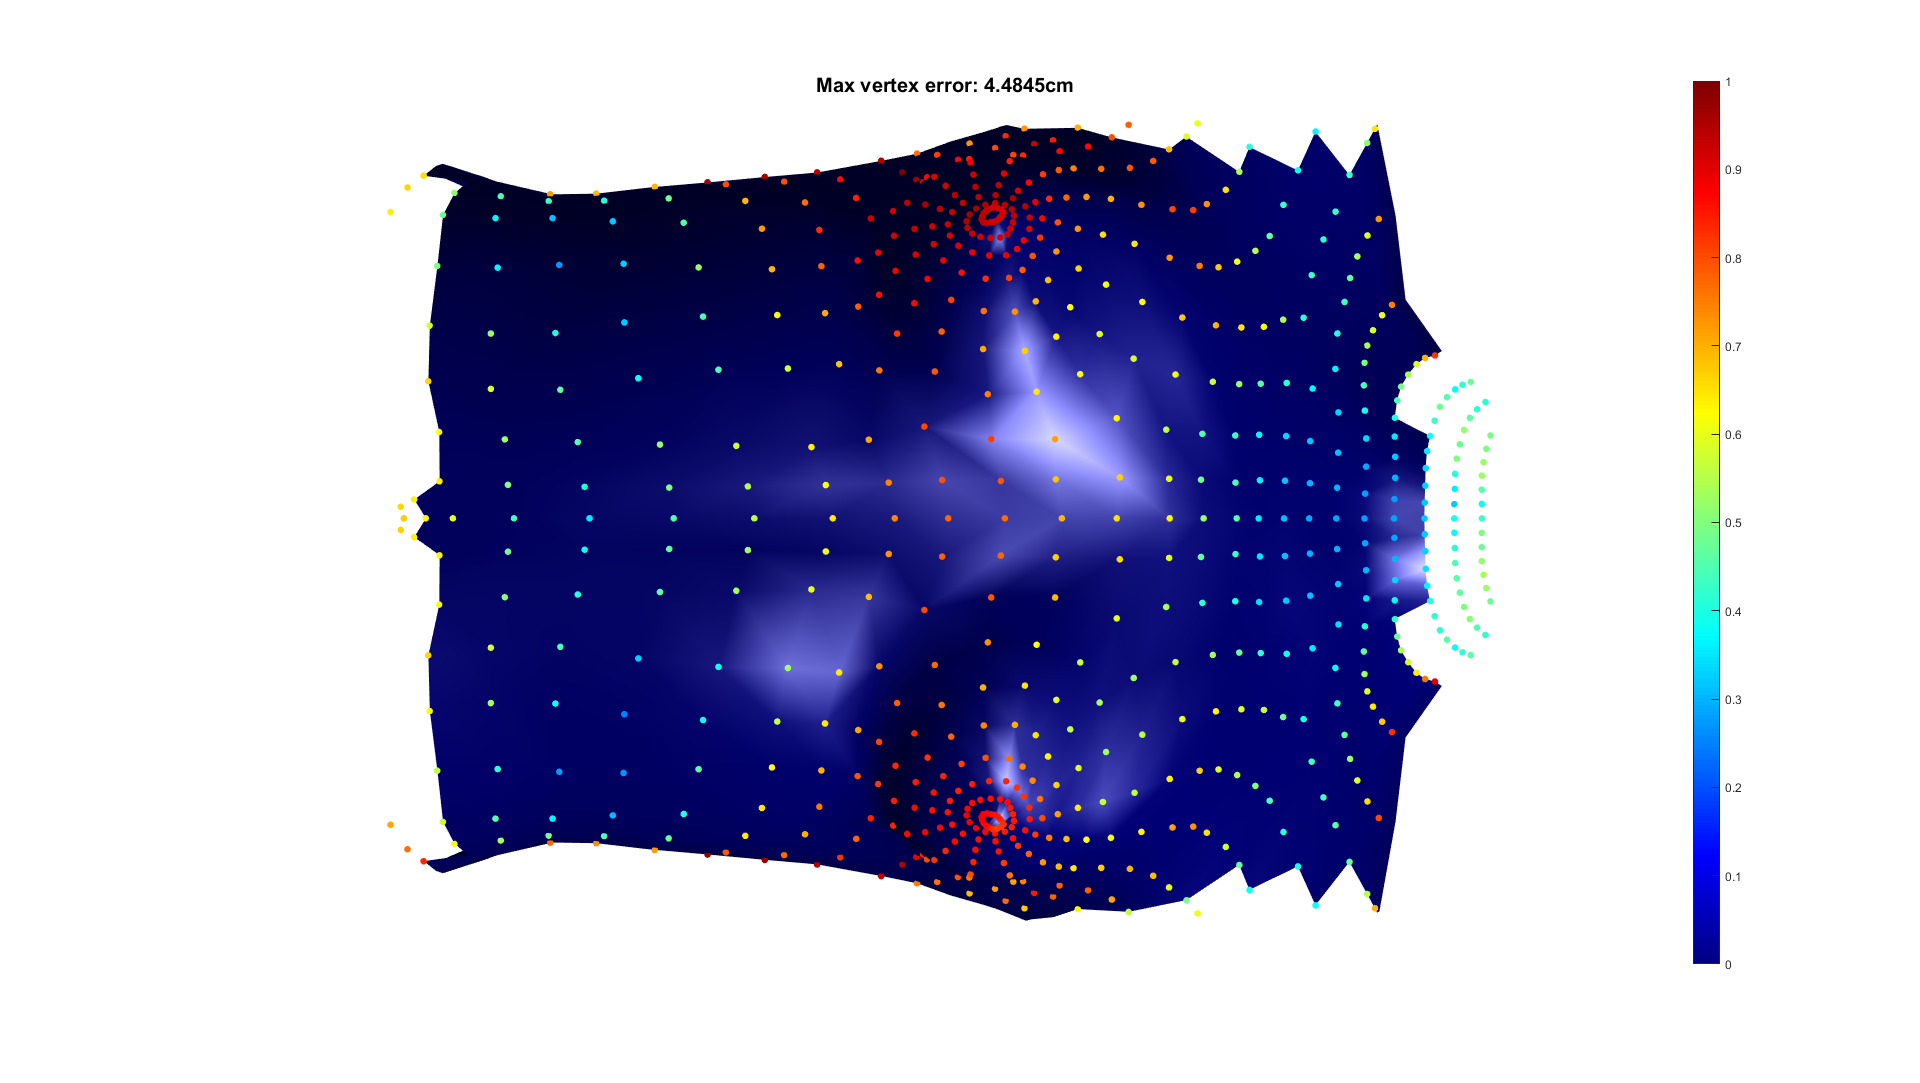
\includegraphics[width=1.1\linewidth]{figures/ceresMhErrorMapBefore}
\end{subfigure}%
\begin{subfigure}{.5\textwidth}
  \centering
  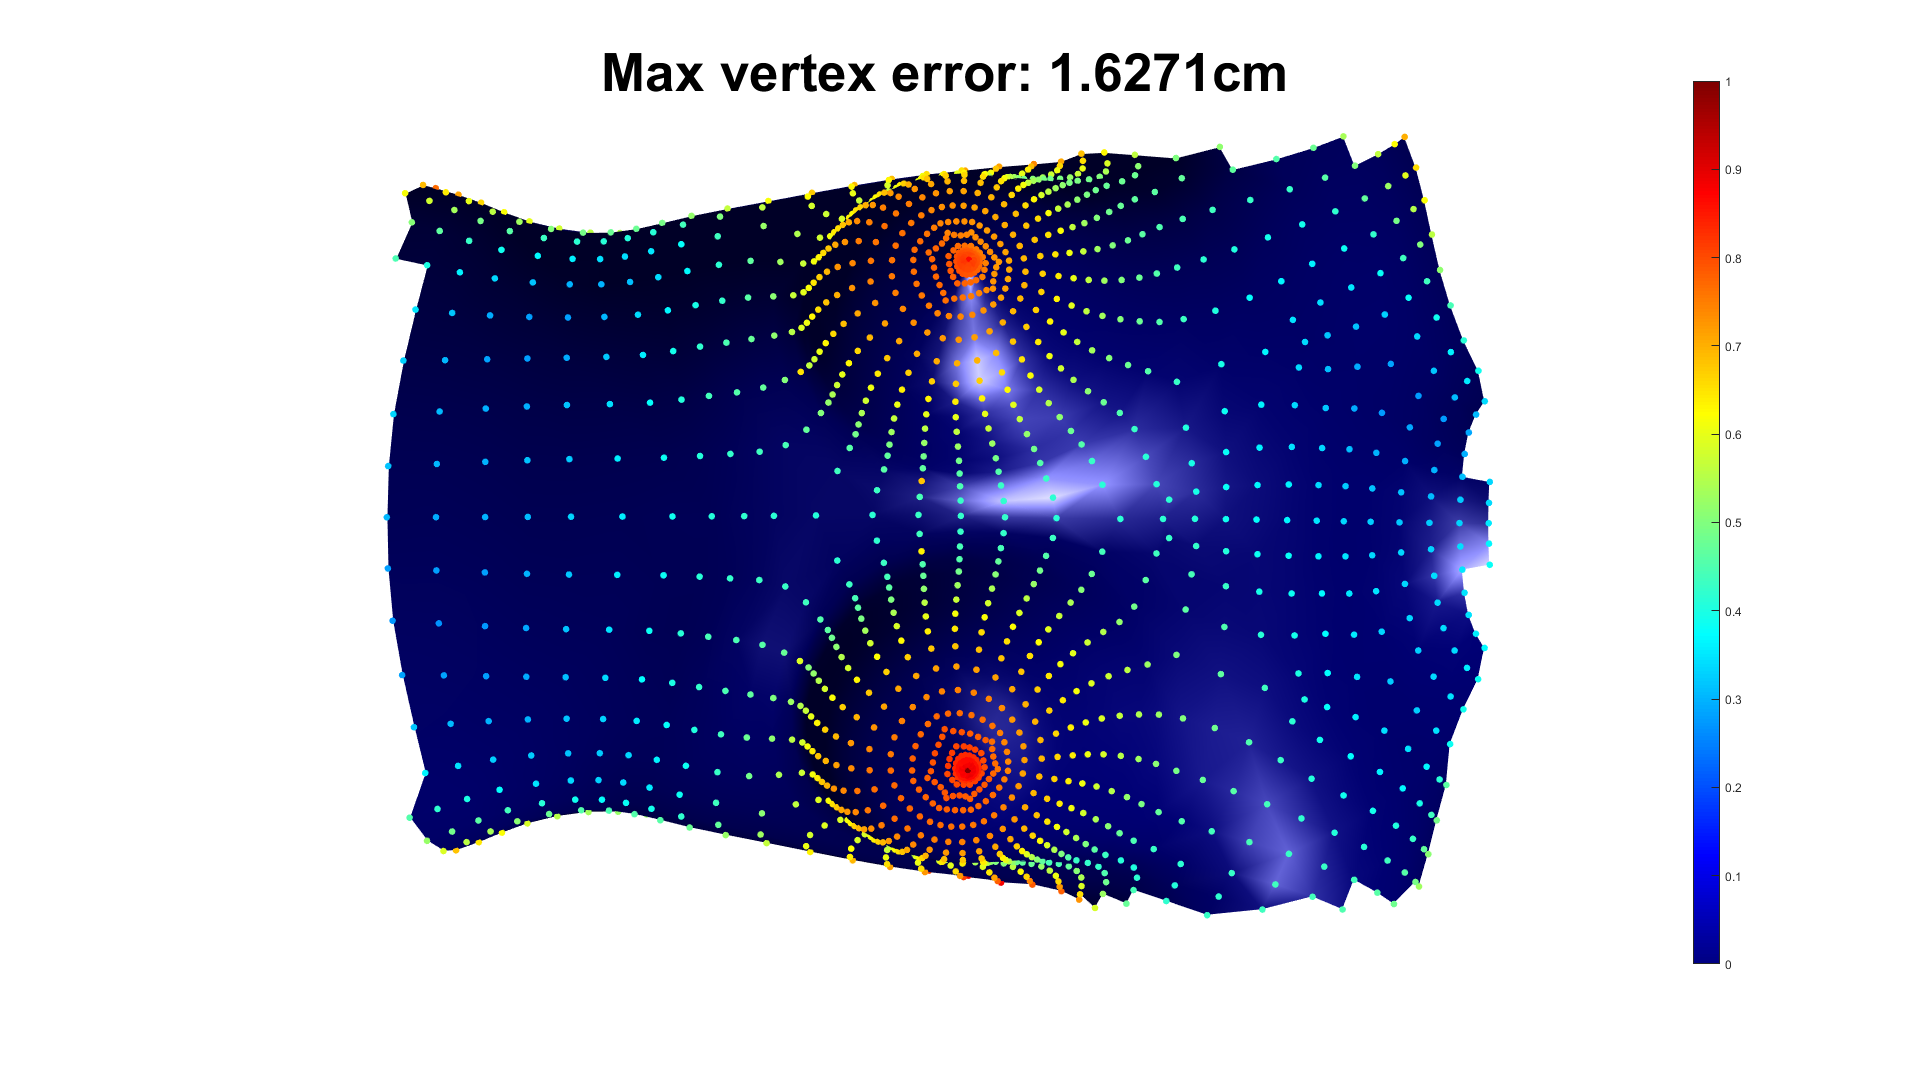
\includegraphics[width=1.1\linewidth]{figures/ceresRealErrorMapBefore}
\end{subfigure}
\caption[Parametric model comparison]{The left image shows the error heat map for the MakeHuman model. The right image depicts the error heat map for the model based on real data.}
\label{fig:compparammodel}
\end{figure}

\subsection{Discussion}
The maximum error for the MakeHuman model is roughly 2.5 times larger than for the real data model. Especially in the nipple area the error is quite large. It appears that this is caused by the difference to the ground truth. When comparing the shape of the MakeHuman ground truth to the input image in figure \ref{fig:compimagefiticp}, it looks like the ground truth solution doesn't represent the input very well. This might be caused by the low resolution of the mesh, hindering the NRICP algorithm from capturing the breast shape features properly. On the other hand, the real data ground truth seems to portray the input image better.\\ The topologies of the meshes are very different. The real data mesh is a lot more refined around the breast and nipple. This leads to a naturally heigher weighting of the breast vertices for the real data model. %TODO

\begin{figure}
\centering
\begin{subfigure}{.22\textwidth}
  \centering
  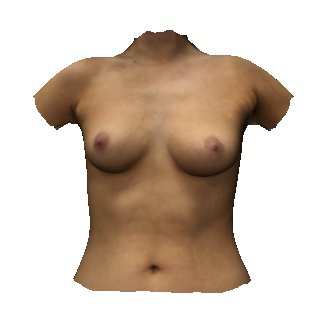
\includegraphics[width=1.05\linewidth]{figures/sprite57}
\end{subfigure}%
\begin{subfigure}{.38\textwidth}
  \centering
  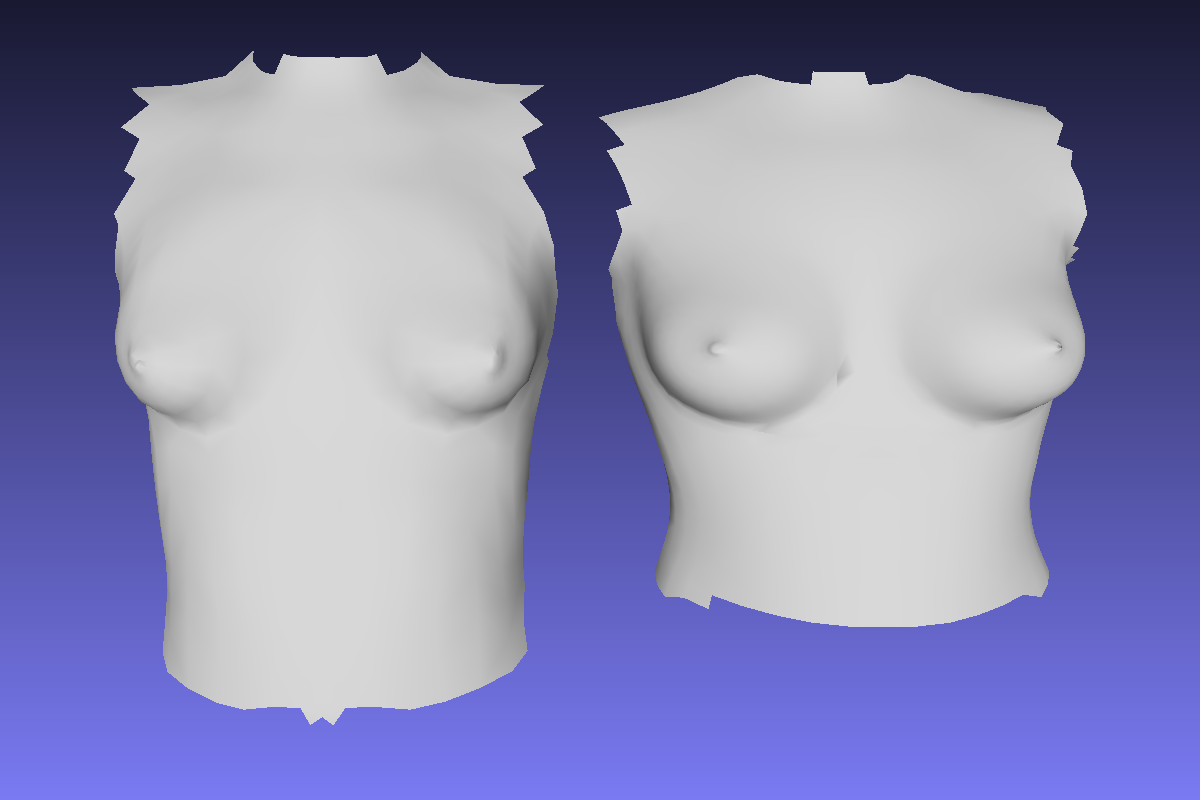
\includegraphics[width=1\linewidth]{figures/fitted57_cropped}
\end{subfigure}
\begin{subfigure}{.38\textwidth}
  \centering
  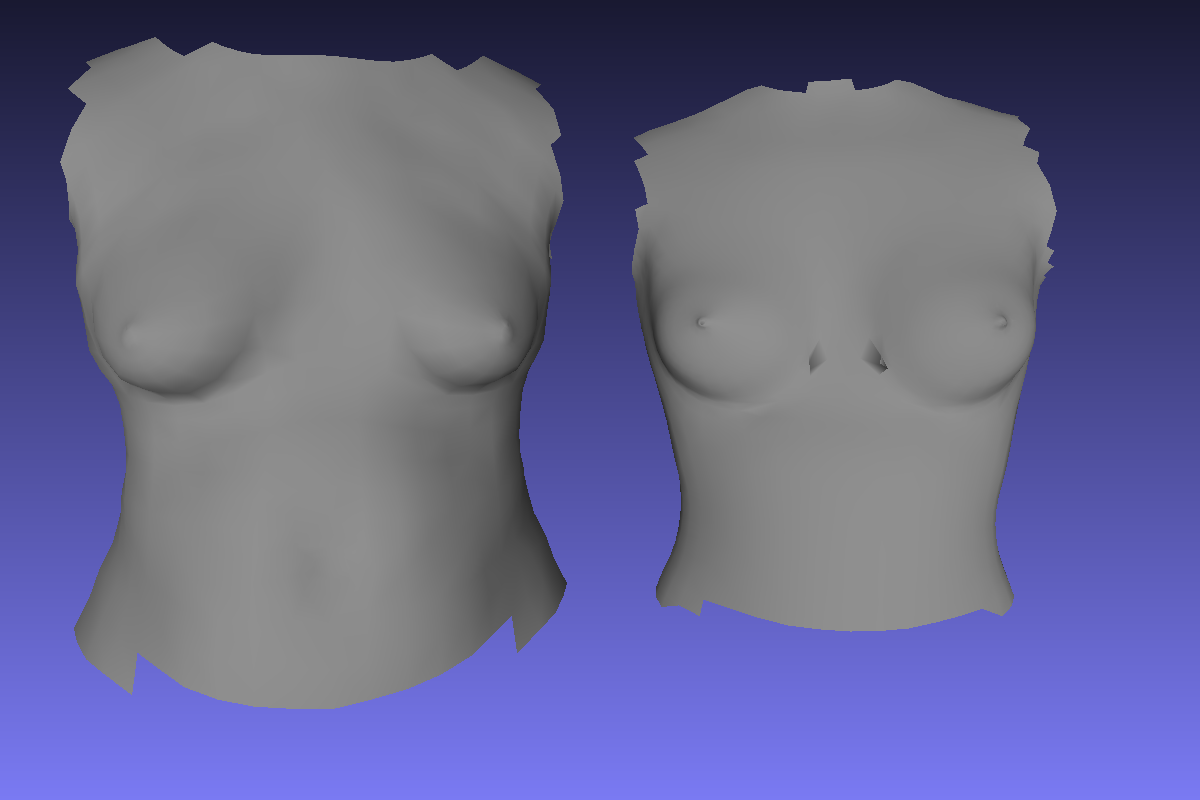
\includegraphics[width=1\linewidth]{figures/before57_cropped}
\end{subfigure}
\caption[Comparison image, fitted and ICP]{The left image shows the torso of the subject. The first two meshes (light grey) are the ground truth meshes, generated from NRICP. The two other meshes (dark grey) are the fits generated by the Ceres implementation. Of each pair, the left mesh represents the MakeHuman model and the right represents the real data model.}
\label{fig:compimagefiticp}
\end{figure}

\chapter{Conclusion}
The first objective of this thesis was to find a mapping between \textit{before} and \textit{after} meshes and explore the possibility of non-linear mappings. It turned out to work quite well using a linear mapping, but the non-linear methods outperformed the linear method completely. Additionally, another model based on triangle deformations was considered and a modification of the point based model, where additional points were generated along the normals of the faces. The point normals method, surprisingly, performed the best, due to the fact that the additional points carried information about triangle surface size, which improves the model. The deformation model doesn't perform as well, as in most cases larger errors occured around the nipple. Perhaps due to the deformation formulation the nipple got slightly misplaced. \\
Lastly, a parametric model based on the MakeHuman editor was compared to a model based on real data. The real data model performed better, due to the fact that the mesh topology was more compatible for the task given. Additionally, that parameteric model was based on similar data. Considering these factors, the parameteric model, based on the editor, performed fairly well.

\section{Outlook}
As most of the tests and experiments were done on considerably small data sets, this is the main point, that could be improved to get more definite results. This could be achieved by using another implementation of SfM or finding better parameters for SfM, such that the reconstruction of the point clouds becomes more successful. Perhaps other data sets would become available, where 3D models are already given and could be used to create a parametric model. \\
Regarding the mappings, the \textit{after} model was only based on a certain label. It would be interesting to explore the relationship between parameters from one model based on, for example, "300" enhancements and "350" enhancements. This could also allow to create intermediate models by interpolating between models. Furthermore, the possibility of using tensorflow instead of scikit-learn could be investigated.\\
The parametric model generated from the MakeHuman meshes could also be further improved, by increasing the number of vertices per mesh. This would require a new implementation for PCA, as the current MATLAB implementation needs too much RAM to be able to load all the meshes and process them for PCA. Another possibility that needs to be explored, would consider to only use breast vertices as correspondences or weight those vertices heigher, due to the fact that the parametric model, generated from the MakeHuman meshes, modifies the complete torso, opposed to the model based on real data, where the most variation already lies in the breasts. This would lead to a better and fairer comparison.



% ---- END MAIN PART ----


\appendix
\clearpage
\renewcommand*{\chapterpagestyle}{myappendixpagestyle}

%\chapter{Appendix}

\begin{table}[]
\centering
\begin{tabular}{lllc}
\cline{2-4}
\multicolumn{1}{l|}{\textbf{PCA}}        & \multicolumn{1}{l|}{\textbf{Method}}        & \multicolumn{1}{l|}{\textbf{Possible Parameters}}                                                                                                           & \multicolumn{1}{c|}{\textbf{Best}} \\ \cline{2-4}
\multicolumn{1}{l|}{\textbf{Incomplete}} & \multicolumn{1}{l|}{\textbf{Random Forest}} & \multicolumn{1}{l|}{'estimator\_\_n\_estimators':{[}5,10,20,30{]},}                                                                                         & \multicolumn{1}{c|}{30}            \\ \cline{2-4}
\multicolumn{1}{l|}{\textbf{}}           & \multicolumn{1}{l|}{\textbf{}}              & \multicolumn{1}{l|}{\begin{tabular}[c]{@{}l@{}}'estimator\_\_max\_features':\\ ('auto', 'sqrt','log2'),\end{tabular}}                                       & \multicolumn{1}{c|}{auto}          \\ \cline{2-4}
\multicolumn{1}{l|}{\textbf{}}           & \multicolumn{1}{l|}{\textbf{}}              & \multicolumn{1}{l|}{'estimator\_\_max\_depth':{[}2,4,8,16{]}}                                                                                               & \multicolumn{1}{c|}{8}             \\ \cline{2-4}
\multicolumn{1}{l|}{\textbf{}}           & \multicolumn{1}{l|}{\textbf{DT}}            & \multicolumn{1}{l|}{'estimator\_\_criterion':('mse','friedman\_mse','mae'),}                                                                                & \multicolumn{1}{c|}{mse}           \\ \cline{2-4}
\multicolumn{1}{l|}{\textbf{}}           & \multicolumn{1}{l|}{\textbf{}}              & \multicolumn{1}{l|}{'estimator\_\_splitter':('random','best'),}                                                                                             & \multicolumn{1}{c|}{best}          \\ \cline{2-4}
\multicolumn{1}{l|}{\textbf{}}           & \multicolumn{1}{l|}{\textbf{}}              & \multicolumn{1}{l|}{'estimator\_\_max\_features':('auto', 'sqrt','log2'),}                                                                                  & \multicolumn{1}{c|}{auto}          \\ \cline{2-4}
\multicolumn{1}{l|}{\textbf{}}           & \multicolumn{1}{l|}{\textbf{}}              & \multicolumn{1}{l|}{'estimator\_\_max\_depth':{[}2,4,8,16{]}}                                                                                               & \multicolumn{1}{c|}{2}             \\ \cline{2-4}
\multicolumn{1}{l|}{\textbf{}}           & \multicolumn{1}{l|}{\textbf{MLP}}           & \multicolumn{1}{l|}{'estimator\_\_activation':('identity','tanh','logistic'),}                                                                              & \multicolumn{1}{c|}{identity}      \\ \cline{2-4}
\multicolumn{1}{l|}{\textbf{}}           & \multicolumn{1}{l|}{\textbf{}}              & \multicolumn{1}{l|}{'estimator\_\_solver':('lbfgs','adam','sgd'),}                                                                                          & \multicolumn{1}{c|}{sgd}           \\ \cline{2-4}
\multicolumn{1}{l|}{\textbf{}}           & \multicolumn{1}{l|}{\textbf{}}              & \multicolumn{1}{l|}{\begin{tabular}[c]{@{}l@{}}'estimator\_\_hidden\_layer\_sizes':\\ {[}(15,),(30,),(45,),(60,),(45,30,),(60,45,){]},\end{tabular}}        & \multicolumn{1}{c|}{(60,45,)}      \\ \cline{2-4}
\multicolumn{1}{l|}{\textbf{}}           & \multicolumn{1}{l|}{\textbf{MLPrelu}}       & \multicolumn{1}{l|}{'estimator\_\_activation':( 'relu'),}                                                                                                   & \multicolumn{1}{c|}{relu}          \\ \cline{2-4}
\multicolumn{1}{l|}{\textbf{}}           & \multicolumn{1}{l|}{\textbf{}}              & \multicolumn{1}{l|}{'estimator\_\_solver':('lbfgs','adam','sgd'),}                                                                                          & \multicolumn{1}{c|}{adam}          \\ \cline{2-4}
\multicolumn{1}{l|}{\textbf{}}           & \multicolumn{1}{l|}{\textbf{}}              & \multicolumn{1}{l|}{\begin{tabular}[c]{@{}l@{}}'estimator\_\_hidden\_layer\_sizes':\\ {[}(15,45,),(45,30,),(60,45,),(60,45,30),(60,45,15){]},\end{tabular}} & \multicolumn{1}{c|}{(45,30,)}      \\ \cline{2-4}
\multicolumn{1}{l|}{\textbf{}}           & \multicolumn{1}{l|}{\textbf{}}              & \multicolumn{1}{l|}{early\_stopping: true}                                                                                                                  & \multicolumn{1}{c|}{true}          \\ \cline{2-4}
\multicolumn{1}{l|}{\textbf{Complete}}   & \multicolumn{1}{l|}{\textbf{RF}}            & \multicolumn{1}{l|}{'estimator\_\_n\_estimators':{[}5,10,20,30{]},}                                                                                         & \multicolumn{1}{c|}{30}            \\ \cline{2-4}
\multicolumn{1}{l|}{\textbf{}}           & \multicolumn{1}{l|}{\textbf{}}              & \multicolumn{1}{l|}{'estimator\_\_max\_features':('auto', 'sqrt','log2'),}                                                                                  & \multicolumn{1}{c|}{auto}          \\ \cline{2-4}
\multicolumn{1}{l|}{\textbf{}}           & \multicolumn{1}{l|}{\textbf{}}              & \multicolumn{1}{l|}{'estimator\_\_max\_depth':{[}2,4,8,16{]}}                                                                                               & \multicolumn{1}{c|}{4}             \\ \cline{2-4}
\multicolumn{1}{l|}{\textbf{}}           & \multicolumn{1}{l|}{\textbf{DT}}            & \multicolumn{1}{l|}{'estimator\_\_criterion':('mse','friedman\_mse','mae'),}                                                                                & \multicolumn{1}{c|}{friedman\_mse} \\ \cline{2-4}
\multicolumn{1}{l|}{\textbf{}}           & \multicolumn{1}{l|}{\textbf{}}              & \multicolumn{1}{l|}{'estimator\_\_splitter':('random','best'),}                                                                                             & \multicolumn{1}{c|}{best}          \\ \cline{2-4}
\multicolumn{1}{l|}{\textbf{}}           & \multicolumn{1}{l|}{\textbf{}}              & \multicolumn{1}{l|}{'estimator\_\_max\_features':('auto', 'sqrt','log2'),}                                                                                  & \multicolumn{1}{c|}{auto}          \\ \cline{2-4}
\multicolumn{1}{l|}{\textbf{}}           & \multicolumn{1}{l|}{\textbf{}}              & \multicolumn{1}{l|}{'estimator\_\_max\_depth':{[}2,4,8,16{]}}                                                                                               & \multicolumn{1}{c|}{2}             \\ \cline{2-4}
\multicolumn{1}{l|}{\textbf{}}           & \multicolumn{1}{l|}{\textbf{MLP}}           & \multicolumn{1}{l|}{'estimator\_\_activation':('identity','tanh','logistic'),}                                                                              & \multicolumn{1}{c|}{tanh}          \\ \cline{2-4}
\multicolumn{1}{l|}{\textbf{}}           & \multicolumn{1}{l|}{\textbf{}}              & \multicolumn{1}{l|}{'estimator\_\_solver':('lbfgs','adam','sgd'),}                                                                                          & \multicolumn{1}{c|}{sgd}           \\ \cline{2-4}
\multicolumn{1}{l|}{\textbf{}}           & \multicolumn{1}{l|}{\textbf{}}              & \multicolumn{1}{l|}{\begin{tabular}[c]{@{}l@{}}'estimator\_\_hidden\_layer\_sizes':\\ {[}(15,),(30,),(45,),(60,),(45,30,),(60,45,){]},\end{tabular}}        & \multicolumn{1}{c|}{(60,45,)}      \\ \cline{2-4}
\multicolumn{1}{l|}{\textbf{}}           & \multicolumn{1}{l|}{\textbf{MLPrelu}}       & \multicolumn{1}{l|}{'estimator\_\_activation':( 'relu'),}                                                                                                   & \multicolumn{1}{c|}{relu}          \\ \cline{2-4}
\multicolumn{1}{l|}{\textbf{}}           & \multicolumn{1}{l|}{\textbf{}}              & \multicolumn{1}{l|}{'estimator\_\_solver':('lbfgs','adam','sgd'),}                                                                                          & \multicolumn{1}{c|}{sgd}           \\ \cline{2-4}
\multicolumn{1}{l|}{\textbf{}}           & \multicolumn{1}{l|}{\textbf{}}              & \multicolumn{1}{l|}{\begin{tabular}[c]{@{}l@{}}'estimator\_\_hidden\_layer\_sizes':\\ {[}(15,45,),(45,30,),(60,45,),(60,45,30),(60,45,15){]},\end{tabular}} & \multicolumn{1}{c|}{(60,45,30,)}   \\ \cline{2-4}
\multicolumn{1}{l|}{\textbf{}}           & \multicolumn{1}{l|}{\textbf{}}              & \multicolumn{1}{l|}{early\_stopping: true}                                                                                                                  & \multicolumn{1}{c|}{true}          \\ \cline{2-4}
                                         &                                             &                                                                                                                                                             & \multicolumn{1}{l}{}
\end{tabular}
\caption[Grid Search parameter table]{The possible parameters were varied to find the best combination. The best option can be seen in the last column.}
\label{gstable}

\end{table}


\clearpage
\renewcommand*{\chapterpagestyle}{empty}

%\nocite{*}
\addcontentsline{toc}{chapter}{Bibliography}
\bibliography{graphics}

\end{document}
